% !TeX program = xelatex 
\documentclass[12pt]{xjtureport}
% =============================================
% Part 0 Edit the info
% =============================================

\name{杨雨潇}
\title{社交网络与文本分析}
\stuid{2201111610}
\class{大数据管理001}
\date{\zhtoday}
\course{社交网络与文本分析}
\instructor{刘跃文}
\expname{课程大作业}
\exptype{设计实验}

\begin{document}
% =============================================
% Part 1 Header
% =============================================
\makecover

% =============================================
% Part 2 Directory
% =============================================
\newpage
\tableofcontents
\setcounter{page}{0}
\thispagestyle{empty}


% =============================================
% Part 3 Main document
% =============================================
% 页眉
\newpage
\pagestyle{fancy}
\fancyhf{} % 清空当前的页眉页脚设置
\renewcommand{\headrulewidth}{0pt} % 设置页眉下划线宽度为 0
\lhead{\itshape 基于漫威宇宙的英雄人物关系分析}
\rhead{\thepage}


\section{基于漫威宇宙的英雄人物关系分析}

\begin{figure}[!htbp]
    \centering
    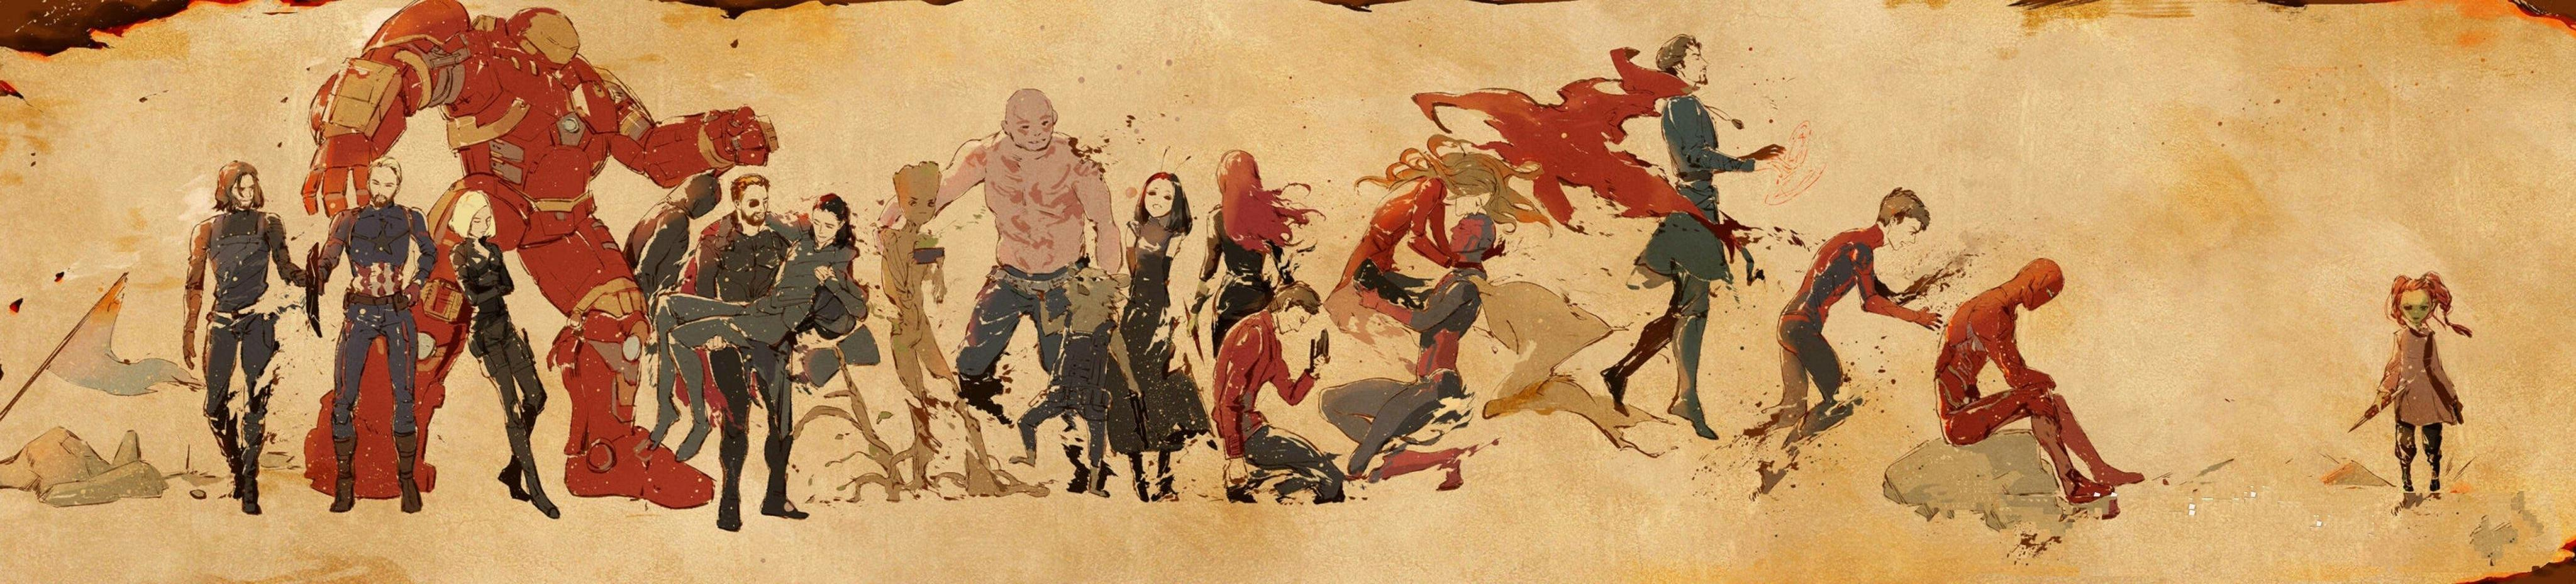
\includegraphics[width=\linewidth]{figures/漫威横幅.jpg}
\end{figure}

\subsection{介绍}

\subsubsection{漫威宇宙介绍}

漫威宇宙是一个由漫威漫画和漫威影业共同创建的虚构世界,其中包含了大量超级英雄和超级反派的故事。漫威宇宙以其丰富的角色设定、复杂的情节和跨影片的连续性而闻名。在漫威宇宙中,存在一种被称为“异变”的现象,它赋予了一些人超凡的能力。这些异变个体中的一些人选择利用他们的能力保护世界,成为超级英雄,而另一些人则利用他们的能力谋取个人利益,成为超级反派。

漫威宇宙中知名的超级英雄有钢铁侠(Iron Man)、美国队长(Captain America)、雷神索尔(Thor)、绿巨人浩克(Hulk)、蜘蛛侠(Spider-Man)和黑寡妇(Black Widow)等。

漫威宇宙还包括一些组织和团队,例如复仇者联盟(Avengers),由一群超级英雄组成,他们联合起来对抗各种威胁。还有X战警(X-Men),由拥有突变基因的超能力人士组成,以及守护者们(Guardians of the Galaxy),一群异星英雄组成的队伍。

\subsubsection{数据来源介绍}

漫威漫画人物合作图最初由巴利阿里群岛大学的Cesc Rosselló、Ricardo Alberich和Joe Miro构建。他们将这个宇宙的特征与现实世界的合作网络进行了比较,比如好莱坞网络,或者由共同撰写研究论文的科学家创建的网络。它们的原始来源可以在\underline{\href{http://bioinfo.uib.es/~joemiro/marvel.html}{这里}}找到。利用这个数据集,作者发表了题为“漫威宇宙看起来几乎像一个真正的社交网络”的论文。本文的研究基础基于前人的归纳整理,在此致谢。


\subsection{人物关系图及基本性质信息}

\begin{figure}[!htbp]
    \centering
    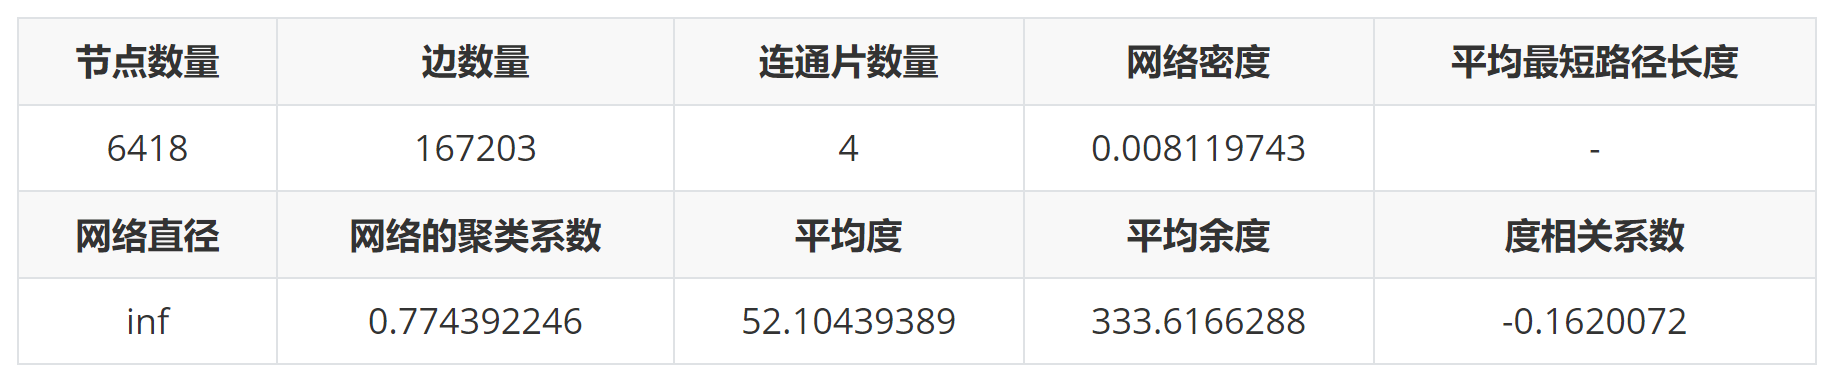
\includegraphics[width=0.9\linewidth]{figures/网络拓扑性质.png}
    \caption{网络拓扑性质}
    \label{attributes}
\end{figure}

由数据集可知,共有漫画12651卷,角色6439个(包含平行宇宙中相同英雄不同人物)。我们对图的定义如下:节点表示不同的角色,若两个节点之间有边相连,则证明两个角色在同一卷漫画中出现过,边的权重以一起出现过的漫画数量表示。网络的示意图如图\ref{T100}所示,相关拓扑结构如图\ref{attributes}所示。

\begin{figure}[!htbp]
    \centering
    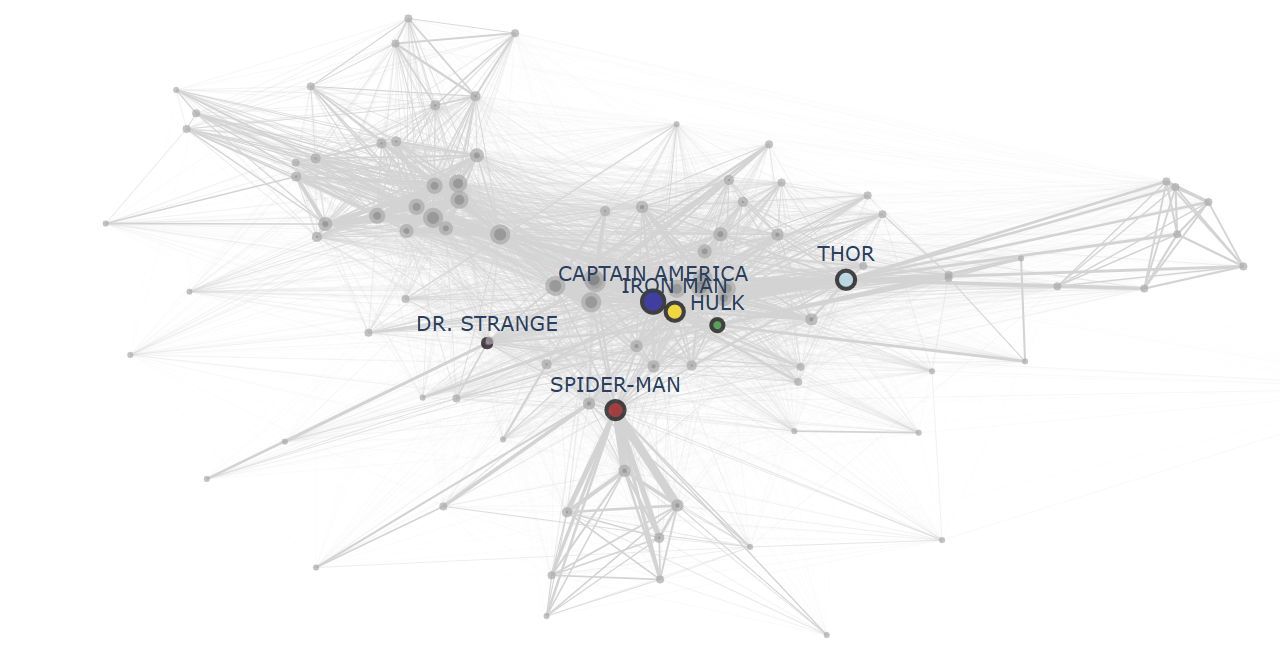
\includegraphics[width=\linewidth]{figures/top 100 Heroes Network.png}
    \caption{排名前100漫威英雄社交网络}
    \label{T100}
\end{figure}

该网络的拓扑性质说明如下:网络的节点数为6418,边数量为167203;网络的连通片数量为4,说明网络不连通,反映出了四个子网络组成;网络密度为0.00812,较为稀疏,反映了网络中实际存在的边数M与最大可能的边数之比;网络的平均最短路径的简谐平均由于计算复杂度过高无法在合理时间内解出,表明社交网络任意两个人物之间联系距离的平均值;网络图的直径由于不连通,为无穷大,它表示网络中任意两个节点之间距离的最大值;网络的聚类系数为0.7743,说明网络的传递性较强,反映了网络中所有节点的聚类系数的平均值;网络的度同配系数为-0.162,表示整个网络呈现异配性,即度大的节点倾向于和度小的节点相连。

网络的平均度为52,平均余度为333。网络的平均度是指网络中每个节点连接的平均数量,而平均余度是指与网络中的每个节点相连的平均节点数(不计重复连接)。这些数据可以反映网络的结构和性质,很好的验证了好友悖论,即大多数人的朋友比他们自己的朋友多。这与网络中的节点连接数量有关,因为每个人的朋友圈往往与节点之间的连接数密切相关。在这种情况下,网络的平均度为52,这意味着每个节点平均连接52个其他节点。而平均余度为333,表示与每个节点相连的平均节点数为333个。

结合好友悖论,可以推断出以下几点:

\begin{enumerate}

    \item 网络中存在一些节点具有非常高的度。由于平均度为52,这意味着大部分节点的度数可能远低于52,而少数节点的度数可能远高于52。这些高度连接的节点可能是网络中的“明星节点”或“超级节点”,与许多其他节点直接相连。

    \item 在网络中,节点之间的连接并不平均。平均余度为333表示与每个节点相连的平均节点数为333个,这表明存在一些节点具有大量的连接,而其他节点可能连接相对较少。这种不平均的连接分布也支持了好友悖论的观察。

    \item 网络中可能存在一些小规模的紧密群体或社区。由于网络的结构可能不均衡,一些节点之间的连接可能更为密集,形成紧密的群体或社区。这些群体内的节点之间的连接可能会增加平均余度,从而导致整体网络的平均余度较高。

\end{enumerate}

网络的度分布呈现幂律分布(如图\ref{degrees});我们进而探索了美国队长(Captain America)的“人脉”,其度为1908,而大多数小角色,度只有两位数,如TAKU,其度为38。

\begin{figure}[!htbp]
    \centering
    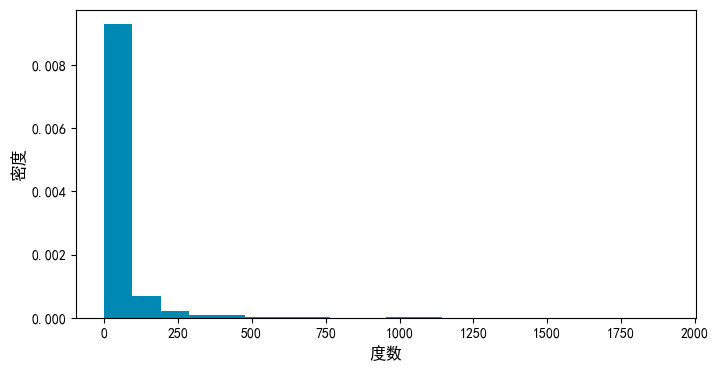
\includegraphics[width=0.8\linewidth]{figures/漫威英雄人物关系度的分布.png}
    \caption{漫威英雄人物关系度的分布}
    \label{degrees}
\end{figure}

\subsection{节点重要性度量}

\subsubsection{指标介绍}
\begin{enumerate}

    \item \textbf{度中心性 Degree Centrality}
    
    度中心性是指归一化的度,若将一个节点连接的边数定义为$k_i$,在一个包含$N$个节点的网络中,节点最大的可能度为$N-1$,可表示为如下式子:
    $$DC_i = \frac{k_i}{N-1}$$
    它体现了某节点的局部重要性或流行性。

    \item \textbf{ 介数中心性 Betweeness Centrality}
    
    一个节点$v$的介数中心性是指图中任意两个节点对之间的最短路径当中,其中经过$v$的最短路径的所占的比例,也就是说经过$v$的最短路径越多,节点$v$越重要。
    $$BC_i = \sum_{s\neq i\neq t}\frac{n^i_{st}}{g_{st}}$$
    其中$g_{st}$为从节点$s$到节点$t$的最短路径的数目,$n^i_{st}$为从节点$s$到节点$t$的$g_{st}$条最短路径中经过节点$i$的最短路径的数目。
    
    一个节点的介性中心度较高,说明其他点之间的最短路径很多甚至全部都必须经过它中转,因此如果这个点消失了,其他点的交流会变得困难。
    
    \item \textbf{接近中心性 CC Closeness Centrality}
    
    接近中心性是一种衡量网络中节点中心性的指标,它是根据节点与图中所有其他节点之间的最短路径长度的倒数来计算的。因此,一个节点越中心,它就越接近所有其他节点。
    $$CC_i = \frac{N-1}{\sum^{N-1}_{j=1}d_{ij}}$$
    其中$d_{ij}$为节点与其它所有节点的平均距离。

    一个点的接近中心度较高,说明该点到网络中其他各点的距离总体来说较近,反之则较远。

    \item \textbf{k-壳与k-核}
    
    K-shell 方法是一种用来划分网络中节点的层次结构的方法,它是根据节点的度来迭代地剥离网络,直到没有节点可以被剥离为止。每个节点被赋予一个 $k$ 值,表示它被剥离时的最小度。具有相同 $k$ 值的节点构成 k-shell。
    
    和度方法不同,k-shell每一步反复循环,直到度等于n的节点全部被移除。
    
    \item \textbf{特征向量中心性 EC Eigenvector Centrality}
    
    特征向量中心性的思路是一个节点的重要性既取决于其邻居节点的数量(度),也取决于邻居节点的重要性。
    $$x = cAx$$
    其中,A是网络的邻接矩阵,x为每个节点的重要性,c为一个比例常数。


    \item \textbf{PR值 PageRank算法}
    
    我们可以通过一个形象的类比来理解PageRank算法,PageRank模拟一个悠闲的上网者,上网者首先随机选择一个网页打开,然后在这个网页上呆了几分钟后,跳转到该网页所指向的链接,这样无所事事、漫无目的地在网页上跳来跳去,PageRank就是估计这个悠闲的上网者分布在各个网页上的概率。
\end{enumerate}

\subsubsection{美国队长真的是队长吗?——节点重要性比较}

\begin{figure}[!htbp]
    \centering
    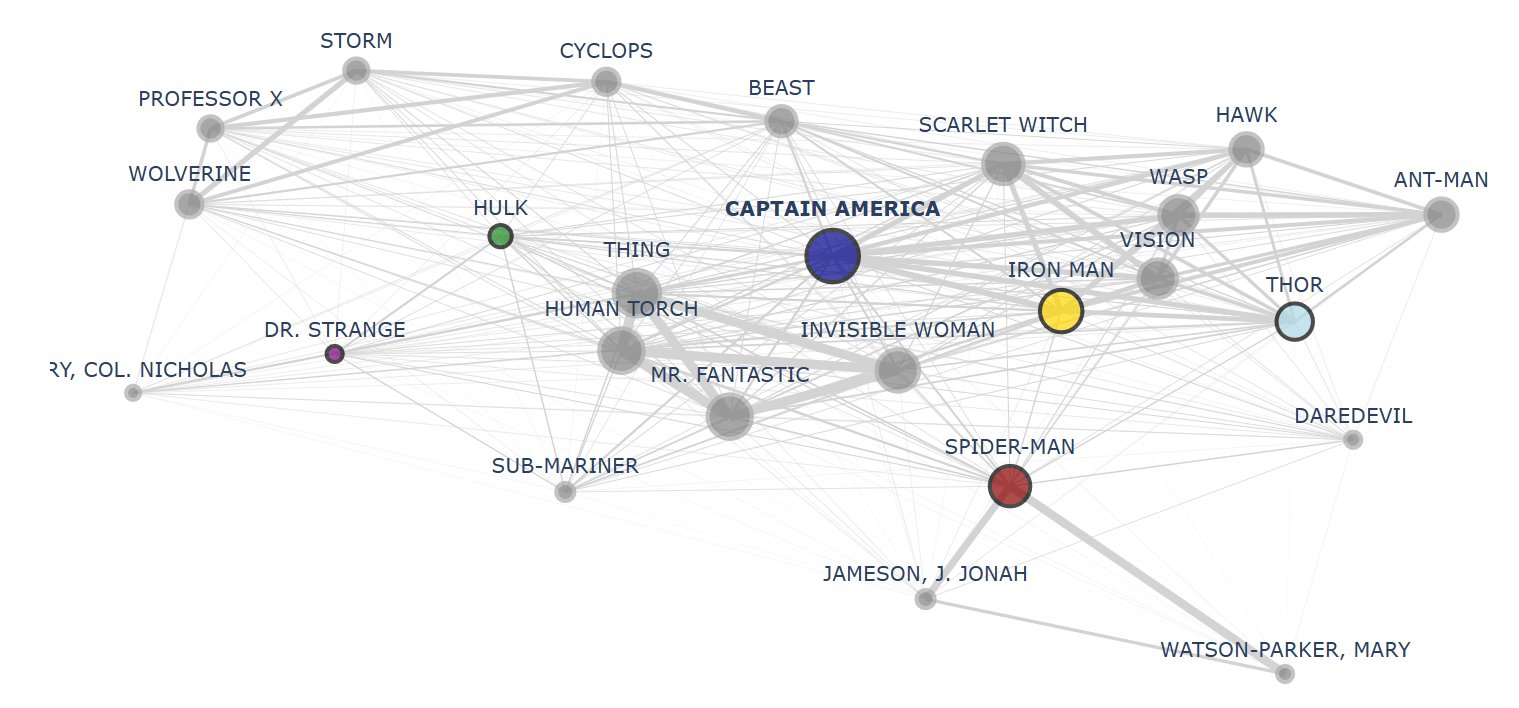
\includegraphics[width=\linewidth]{figures/top 25 Heroes Network.png}
    \caption{排名前25漫威英雄社交网络}
    \label{T25}
\end{figure}

由于全图权重的计算复杂度较高,我们依据在漫画中出现的次数排序,选取了出现频率最高的前25个英雄,以进行局部角色细节的分析。其中,节点表示英雄,节点的大小表示中心性(基于PR值),边的权重用一起出现过的漫画数量表示,某些很著名的超级英雄用特定的颜色标记美国队长、钢铁侠、蜘蛛侠、巨人、托尔、奇异博士,具有最高中心性的以粗体标记,如图\ref{T25}。

该社交网络为全连接,即密度为1,平均最短路径长度为1,聚类系数为1,由社交网络图我们可以得到以下结论:

\begin{enumerate}
    \item 你可以在右上角看到电影《复仇者联盟》中的英雄们。

    \item 你可以在中心看到神奇四侠之间的紧密联系。

    \item 在右下角,蜘蛛侠周围的人物与蜘蛛侠有着紧密的联系。
\end{enumerate}

\begin{figure}[!htbp]
    \centering
    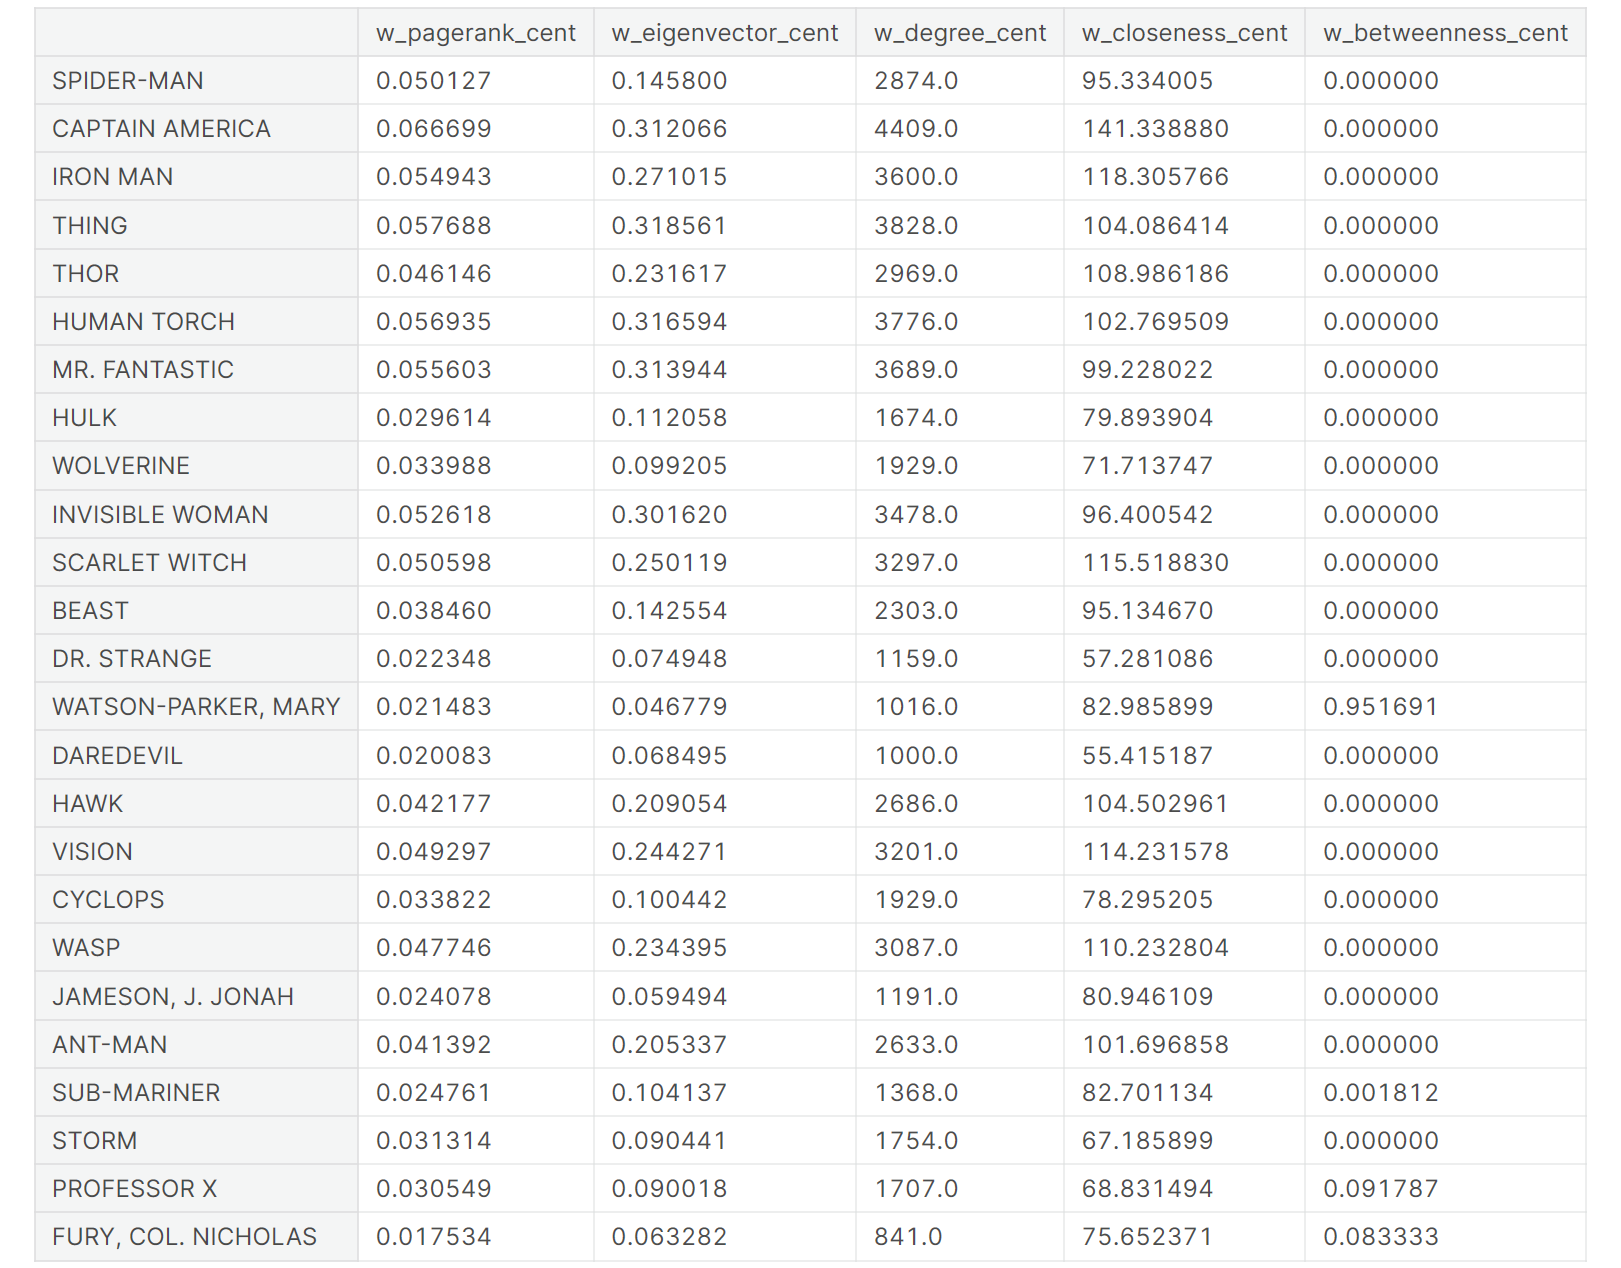
\includegraphics[width=\linewidth]{figures/中心度可视化.png}
    \caption{各英雄中心度值}
    \label{central}
\end{figure}

各英雄基于各种中心度测量方式的计算值如图\ref{central},我们可以得到以下分析结果:

\begin{enumerate}
    \item 因为所有英雄都是相互关联的,所以考虑介数中心性 Betweenness Centrality是不合适的。
    \item 因为每个中心性都有不同的尺度,所以有必要统一范围进行比较,即进行标准化。
    \item 经过MinMaxScaler中心化后,将四种中心性度量取平均值作为最终中心度的衡量标准。
\end{enumerate}

\begin{figure}[!htbp]
    \centering
    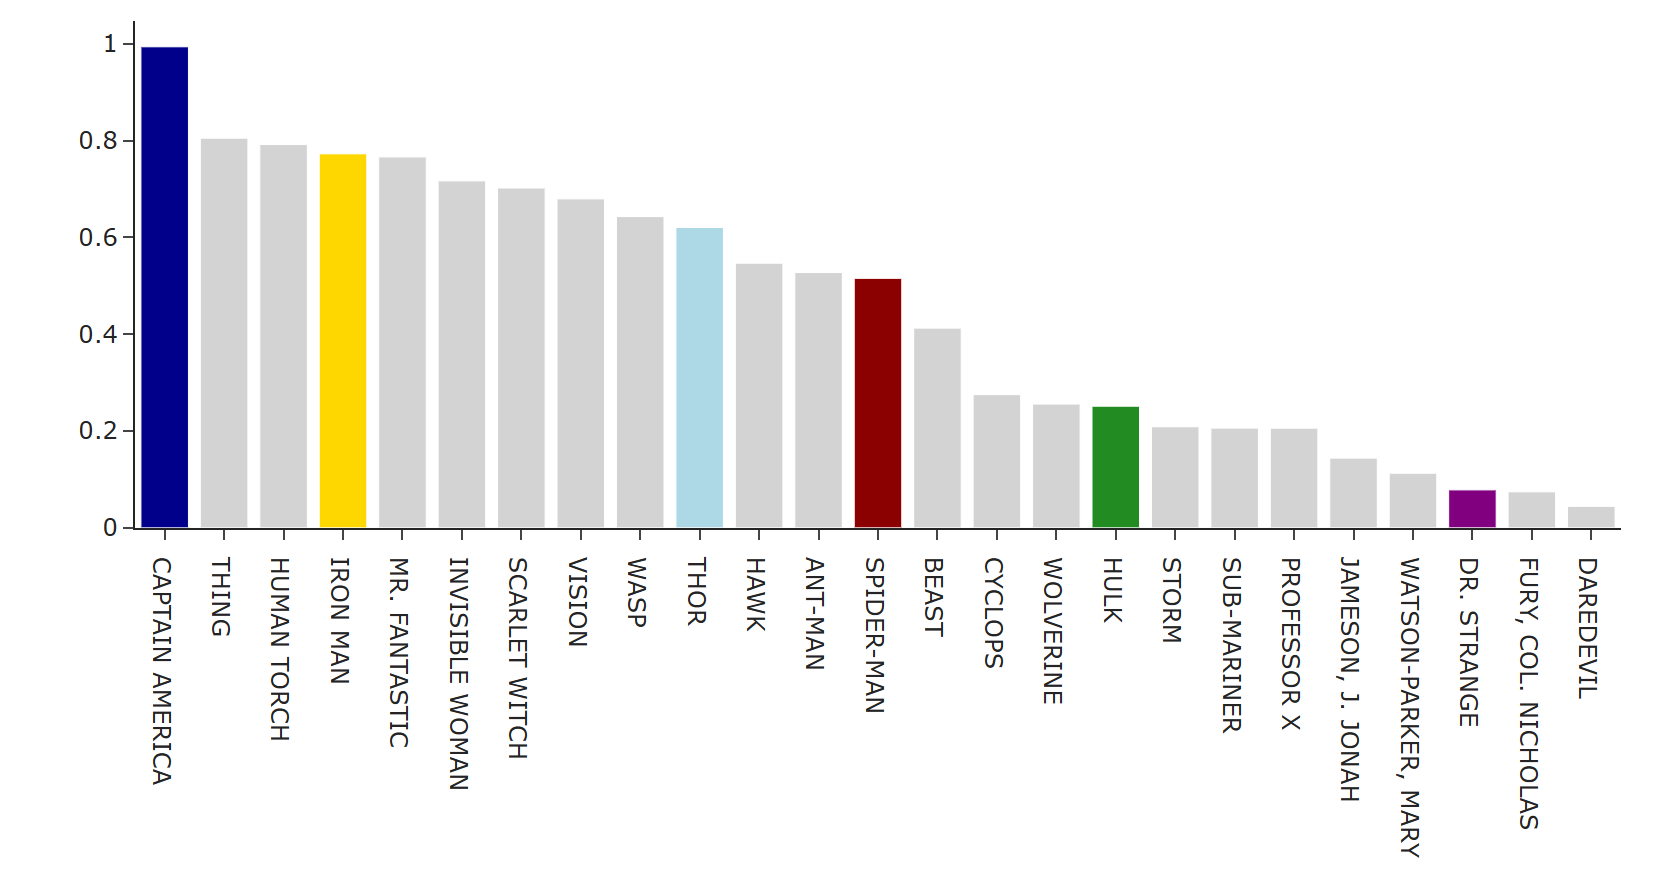
\includegraphics[width=\linewidth]{figures/平均中心度可视化.png}
    \caption{各英雄平均中心度}
    \label{central_mean}
\end{figure}



在计算并排序了平均中心性之后(见图\ref{central_mean}),我们发现美国队长的平均中心度最高,接近1,\textbf{美国队长就是队长}!

\subsubsection{灭霸打响指之后——角色重要性演变}
在灭霸打响指之前,我们探究一下规模变大是否会影响某个英雄所处的地位吗?其重要性会发生怎样的变化?为了探究规模对角色重要性的影响,我们进而选取了Top50,Top100,Top200,Top500的数据进行测试,结果如下(见图\ref{fig:combined}):
\begin{figure}[htbp]
    \centering
    \begin{subfigure}[b]{0.3\textwidth}
      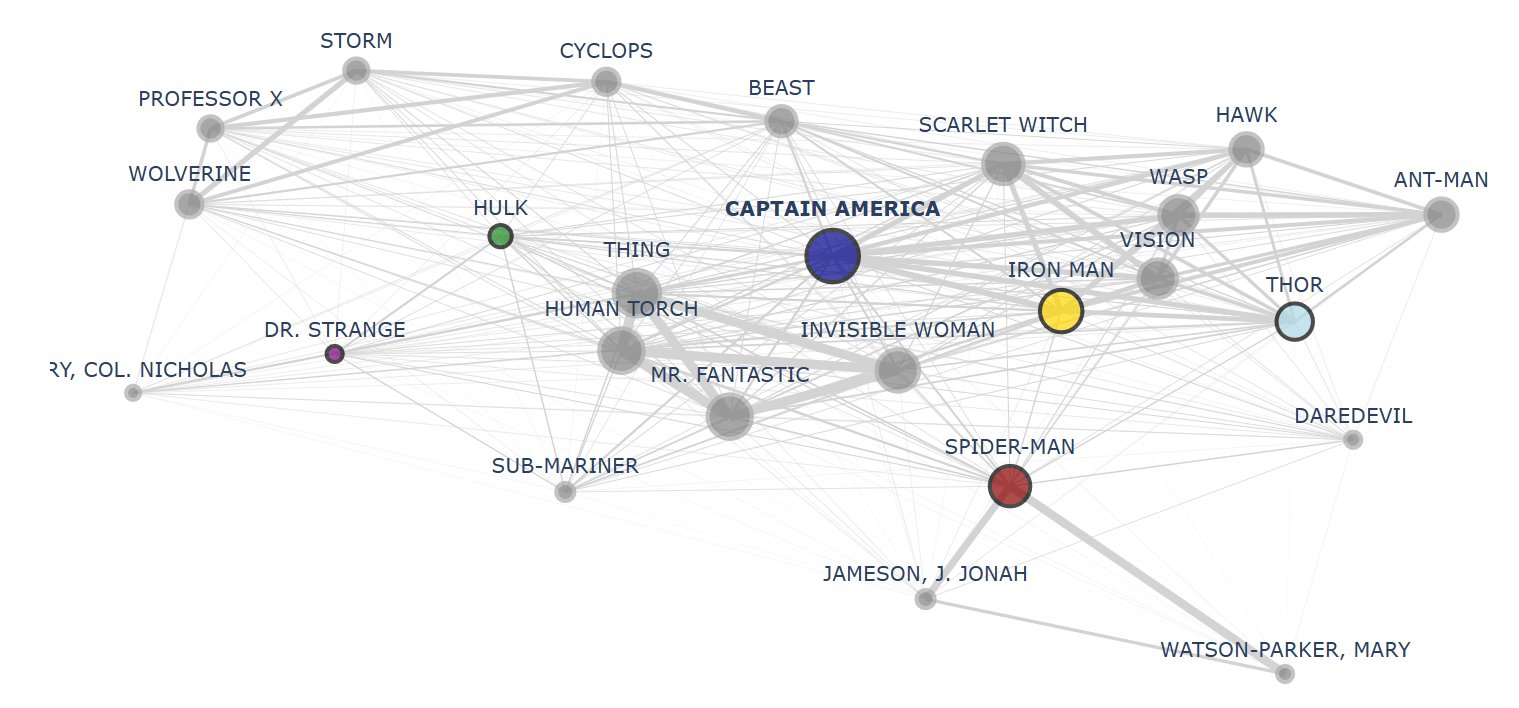
\includegraphics[width=\textwidth]{figures/top 25 Heroes Network.png}
      \caption{Top 25}
      \label{fig:sub1}
    \end{subfigure}
    \hfill
    \begin{subfigure}[b]{0.3\textwidth}
      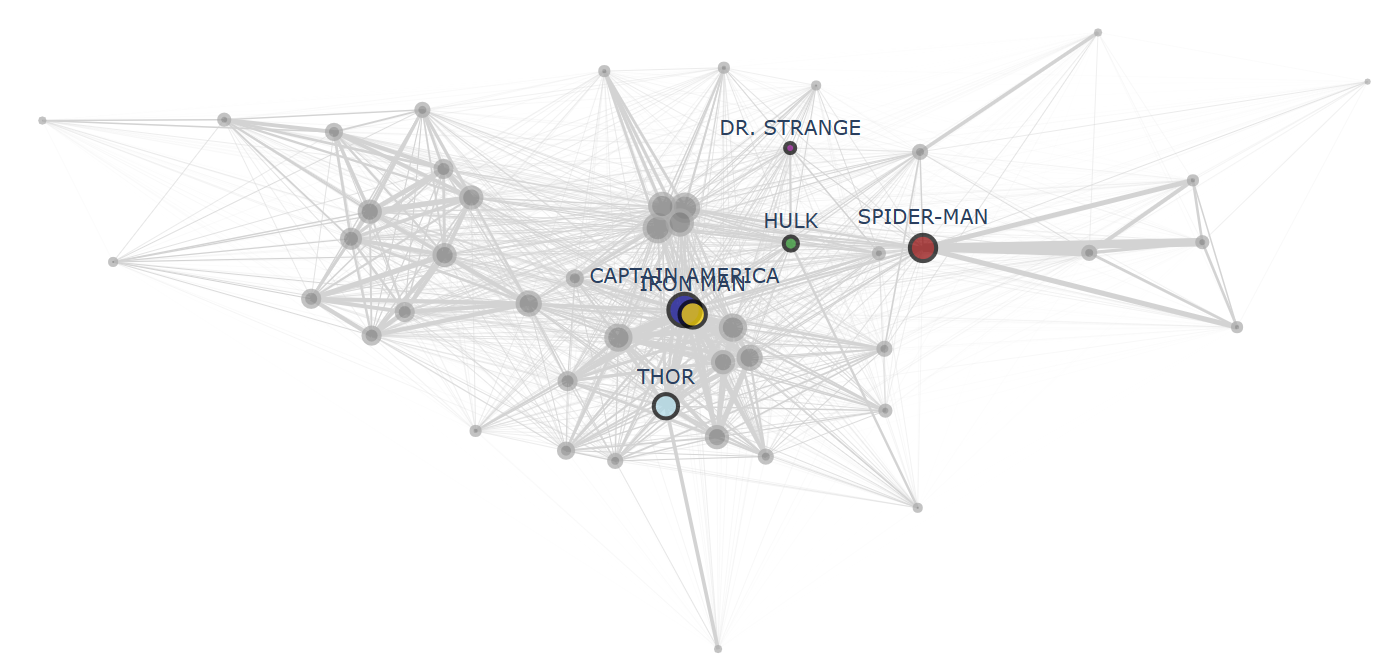
\includegraphics[width=\textwidth]{figures/top 50 Heroes Network.png}
      \caption{Top 50}
      \label{fig:sub2}
    \end{subfigure}
    \hfill
    \begin{subfigure}[b]{0.3\textwidth}
      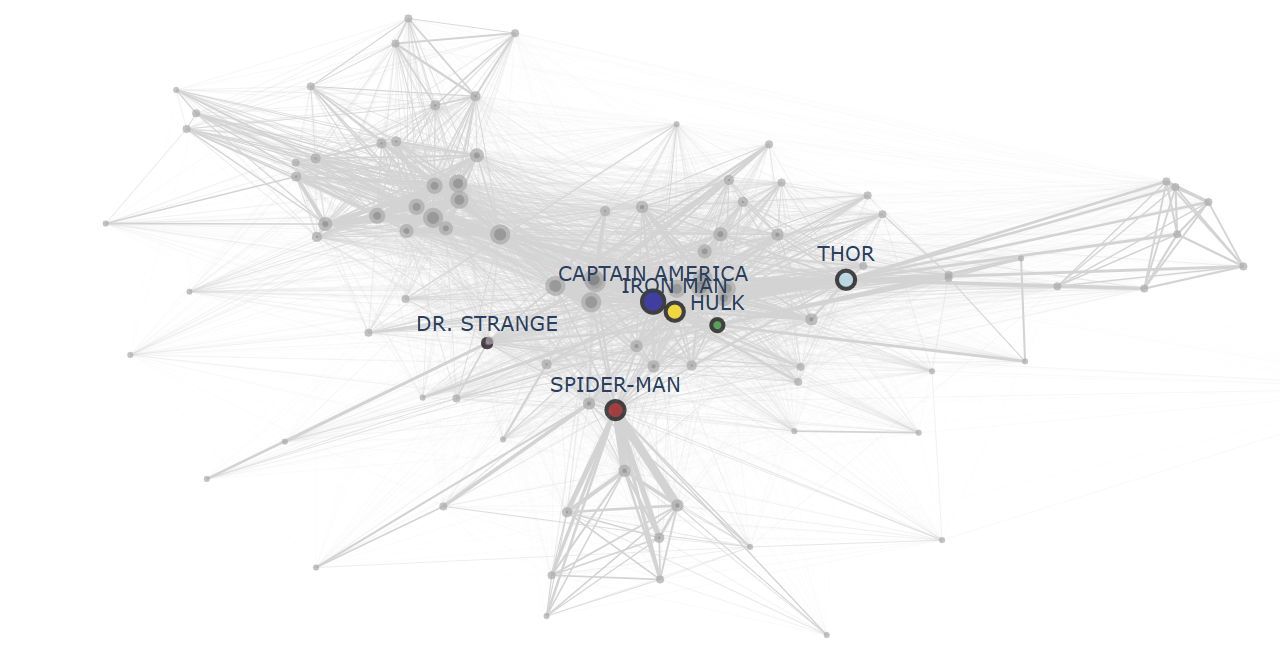
\includegraphics[width=\textwidth]{figures/top 100 Heroes Network.png}
      \caption{Top 100}
      \label{fig:sub3}
    \end{subfigure}
    \caption{英雄规模为25 50 100 的网络结构对比}
    \label{fig:combined}
  \end{figure}

我们可以发现美国队长的排名看起来相当高(所有网络中的节点都相当大);并且随着英雄数量的增加,似乎存在连接较弱的英雄(网络中的节点与其他节点联系不紧密)。

\begin{figure}[!htbp]
    \centering
    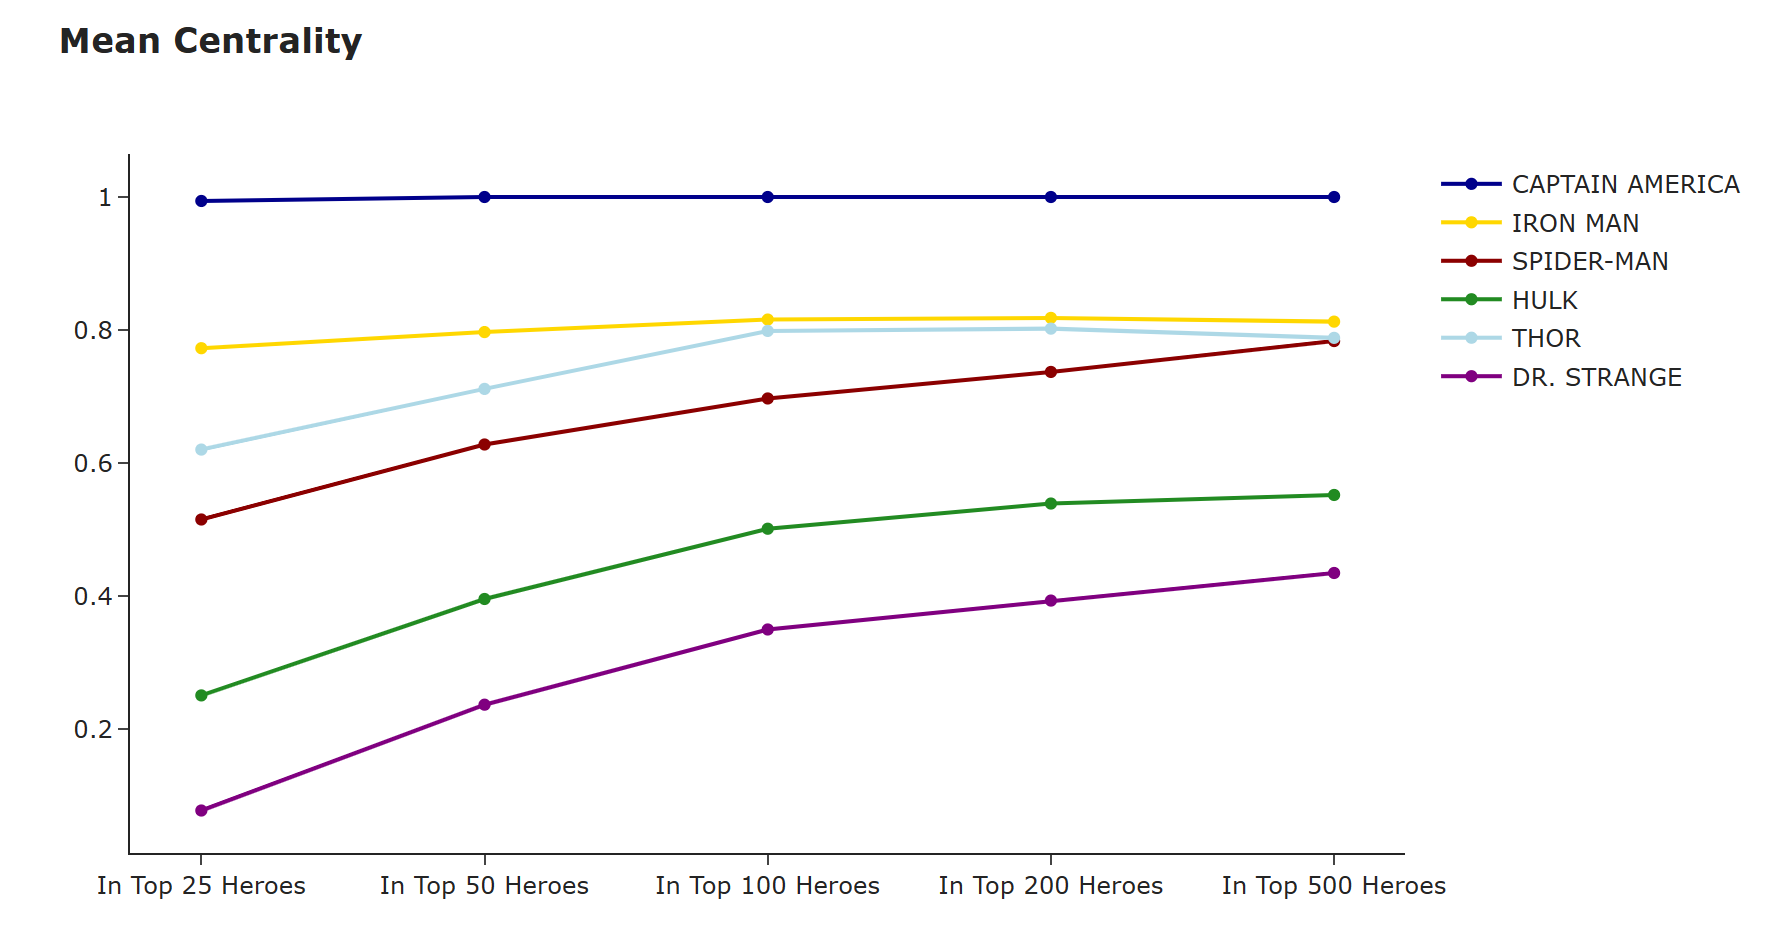
\includegraphics[width=\linewidth]{figures/不同英雄规模下的平均中心度.png}
    \caption{不同规模下各英雄的平均中心度}
    \label{central_mean_nums}
\end{figure}

通过分析不同英雄规模下的平均中心度(见图\ref{central_mean_nums}),我们可以得到以下推论:

\begin{enumerate}
    \item 有些英雄无论英雄数量多少,都会保持很高的中心性和重要性,如美国队长,铁人。不管其他英雄的认可程度如何,他们在都是较为优秀、积极、存在感高的英雄。

    \item 随着英雄数量的增加,有些英雄的平均中心性也会增加,如蜘蛛侠,奇异博士。他们的重要程度随着英雄规模的增大而不断增大,说明其能力还是较为关键的。
\end{enumerate}

灭霸的响指即将降临,会对我们英雄的中心性造成什么样的变化呢?在漫威电影中,灭霸用手指拍下了整个宇宙中一半的生命。一半的英雄随着他的手指弹消失了,让我们看看英雄网络上发生了什么变化。
\begin{figure}[b]
    \centering
    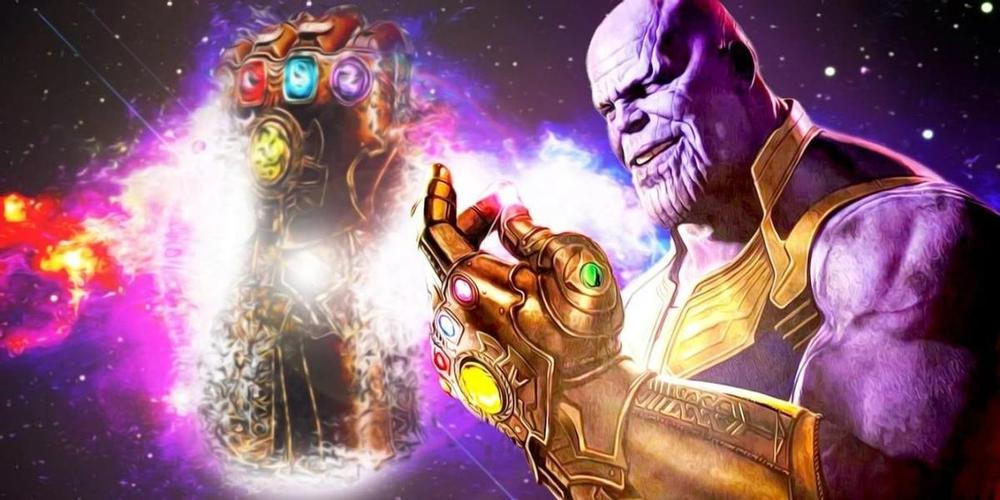
\includegraphics[width=0.7\linewidth]{figures/灭霸打响指.jpeg}
    \caption{灭霸打响指}
    \label{dimo}
\end{figure}
考虑一个由100位英雄组成的网络,对打响指前后进行比较。然后我们假设消失一半的节点是随机的。如果是这样的话,响指之后的网络会与现有的50英雄网络有相似的特征吗?

\begin{figure}[htbp]
    \centering
    \begin{subfigure}[b]{0.49\textwidth}
        \centering
        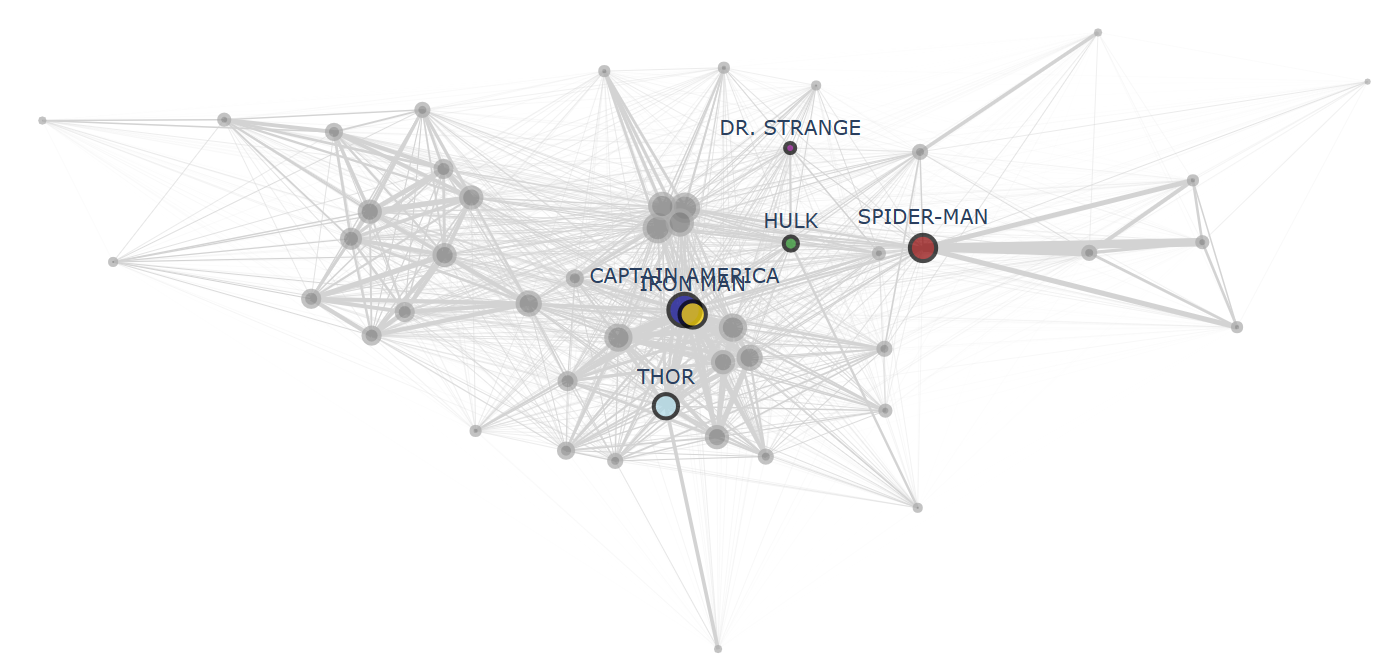
\includegraphics[width=\linewidth]{figures/top 50 Heroes Network.png}
        \caption{Top50英雄网络}
        \label{fig:sub11}
        \end{subfigure}
        \hfill
    \begin{subfigure}[b]{0.49\textwidth}
        \centering
        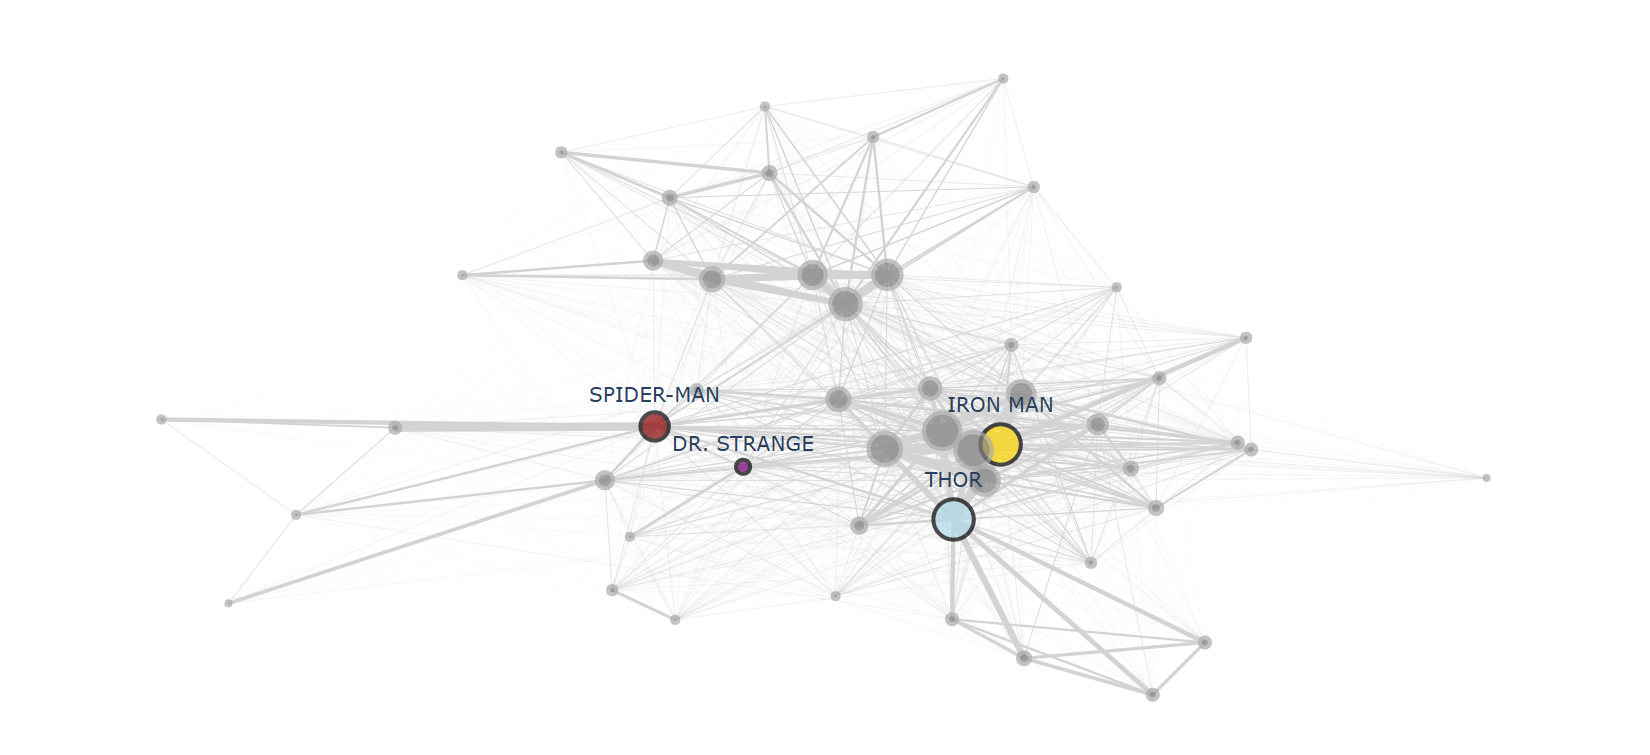
\includegraphics[width=\textwidth]{figures/响指过后top 50 Heroes Network.png}
        \caption{响指后Top50英雄网络}
        \label{fig:sub22}
    \end{subfigure}
    \caption{响指过后网络结构前后对比}
    \label{fig:combined2}
  \end{figure}
  

该网络(见图\ref{fig:combined2})是在灭霸打响指之后的网络。美国队长和绿巨人浩克因为响指而消失了。响指过后的50英雄网络与现有的50英雄网络相比,连接似乎明显减少。

\begin{figure}[htbp]
    \centering
    \begin{subfigure}[b]{0.35\textwidth}
        \centering
        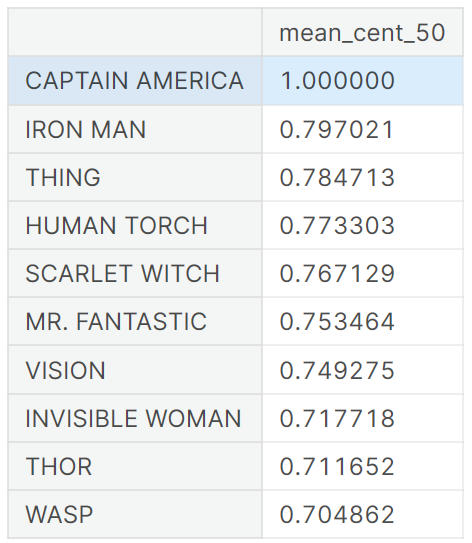
\includegraphics[width=\linewidth]{figures/响指前top10.png}
        \caption{响指前Top10英雄中心度得分}
        \label{fig:sub13}
        \end{subfigure}
    \hspace{0.1\textwidth} % 调整两张图片之间的间距
    \begin{subfigure}[b]{0.35\textwidth}
        \centering
        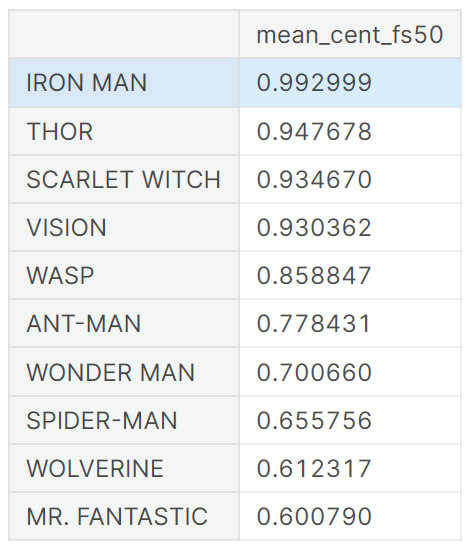
\includegraphics[width=\textwidth]{figures/响指后top10.png}
        \caption{响指后Top10英雄中心度得分}
        \label{fig:sub23}
    \end{subfigure}
    \caption{响指过后英雄中心度得分前后对比}
    \label{fig:combined3}
  \end{figure}

上述表格(见图\ref{fig:combined3})显示了每个网络中基于中心性的前10名英雄,响指过后,我们可以得到以下分析结果:
\begin{enumerate}
    \item 新队长是钢铁侠。
    \item 雷神索尔和绯红女巫位居榜首。
    \item 奇异博士的中心地位比以前低了。
\end{enumerate}

\subsection{节点相似性度量}
\subsubsection{基于局部信息的节点相似性指标}
共同好友/共同领域 Common Neighbors

社会网络分析中三元闭包(Triadic closure)原则指出,如果两个人A和B拥有一个共同的朋友C,那么这两个人今后也很有可能成为朋友,从而使三个节点构成一个闭合的三角形ABC。

对于一般的网络,这一原则推广如下:如果两个节点的共同邻居的数量越多,这两个节点就越相似,从而更倾向于互相连接。

$$S_{xy}^{CN} = |\Gamma(x) \cap \Gamma(y)|$$

Adamic-Adar(AA)指标是对共同好友进行加权后的指标,是非常经典的指标,计算公式如下:

$$S_{xy}^{AA} = \sum_{z \in \Gamma(x) \cap \Gamma(y)}\frac{1}{log k(z)}$$

下面取钢铁侠为例,利用AA指标为其推荐好友,见图\ref{friend1}:

\begin{figure}[!htbp]
    \centering
    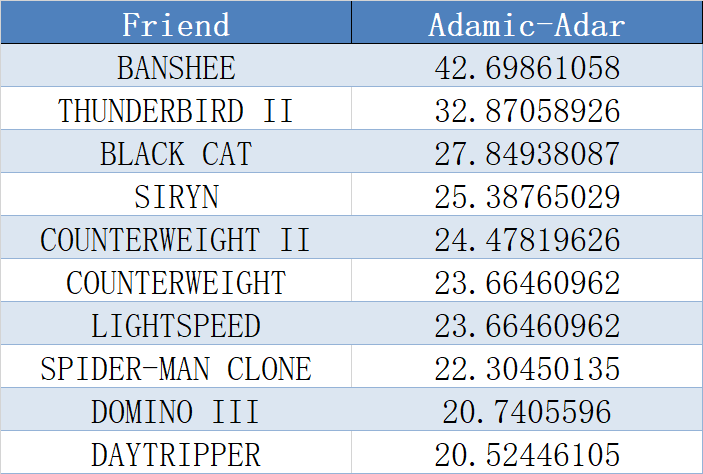
\includegraphics[width=0.5\linewidth]{figures/钢铁侠推荐好友.jpg}
    \caption{基于AA指标为钢铁侠推荐好友}
    \label{friend1}
\end{figure}

我们可以发现,钢铁侠最应该认识海妖(BANSHEE),海妖初次登场于《X战警》(X-Men)第28期(1967年一月),由Roy Thomas和以及Werner Roth创造。本名西恩·卡西迪(Sean Cassidy),是X战警成员。第二名是雷鸟(Thunderbird),初次登场于《Giant-Size X-Men》第1期(1975年5月)。本名约翰·普罗德斯达(John Proudstar),是X战警成员。第三名是黑猫(BLACK CAT),初次登场于《神奇蜘蛛侠》(The Amazing Spider-Man)第194期(1979年7月),由编剧Marv Wolfman和画师Keith Pollard创造,是大盗灵猫(The Cat)的女儿,蜘蛛侠的搭档。

\subsubsection{基于全局信息的节点相似性指标}

对于矩阵表示法的理解:

矩阵的元素$A_{ij}$表示两个节点$i$与$j$之间是否有一步通路。显然,自己和自己之间不可能有一步通路(除非有自环),因此对角线为0。

矩阵的元素$A_{ij}^{2}$表示两个节点$i$与$j$之间是否有两步通路。

$\bullet$显然,自己和自己之间一定有两步通路(自己-好友-自己),通路数正好为好友数,对角线为好友数。从矩阵乘法上来看,就是自己连接别人的向量,与别人连接自己的向量的乘法,很显然,有好友的地方才能对应上。

$\bullet$自己和别人连接的两步通路为(自己-好友-二度好友),通路数正好为二度好友数。从矩阵乘法上来看,就是自己连接别人的向量,与别人连接目标的向量的乘法,只有不为零元素对应上(中间有共同好友),才会被计算进来。

矩阵的元素$A_{ij}^{3}$表示两个节点$i$与$j$之间是否有三步通路。

以此类推,矩阵的元素$A_{ij}^{n}$表示两个节点$i$与$j$之间是否有n步通路。

基于以上理解,表达出漫威宇宙英雄人物关系的矩阵二步通路(见图\ref{222}),其矩阵维度为(6418, 6418):

\begin{figure}[!htbp]
    \centering
    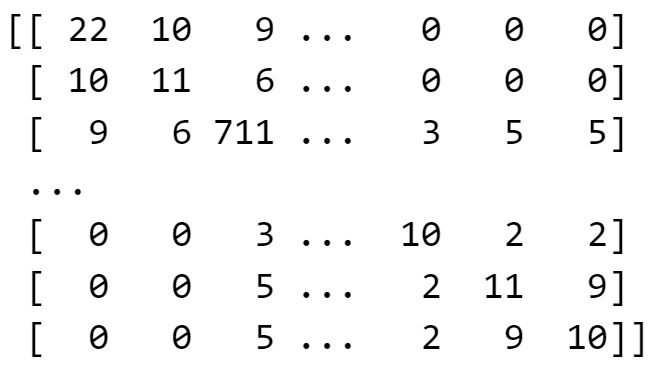
\includegraphics[width=0.4\linewidth]{figures/全局信息表示.jpg}
    \caption{全局信息二步通路矩阵表示}
    \label{222}
\end{figure}

\subsubsection{基于随机游走的相似性指标}

PageRank算法是一种用于确定网络图中节点重要性的算法,它通过迭代计算节点之间的链接关系来确定节点的排名。PageRank 的计算方法有多种实现方式,其中 $pagerank_numpy()$ 使用了基于矩阵运算的方法来实现。

下面同样取钢铁侠为例,利用PageRank算法计算其好友关系:

\begin{figure}[!htbp]
    \centering
    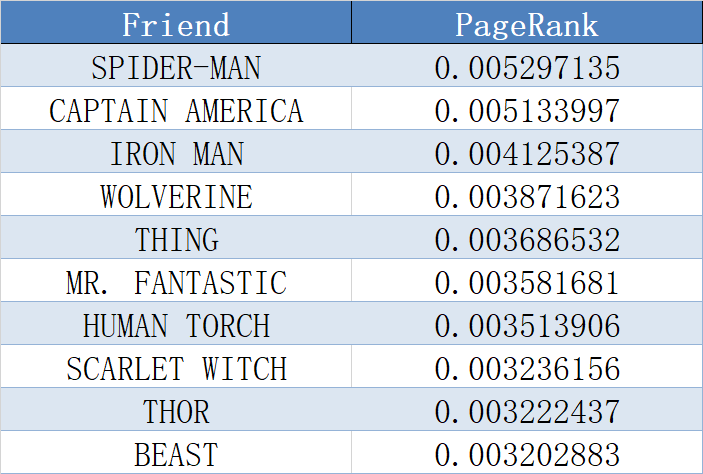
\includegraphics[width=0.5\linewidth]{figures/钢铁侠推荐好友2.jpg}
    \caption{钢铁侠基于PR值的好友关系}
    \label{friend2}
\end{figure}

我们从表格可以看出,钢铁侠与蜘蛛侠关系最好,钢铁侠在电影剧情中作为是拉蜘蛛侠进入复仇者联盟的人,基本可以对蜘蛛侠来说是属于“亦父亦友”的存在。

\subsection{我们属于同一个联盟吗?——社团识别}

本文基于三种不同的社团识别算法来进行社团划分,分别是Q贪婪算法、louvain算法和KMeans算法,并对比三种算法的时间和空间复杂度,下面是三种算法简单的介绍:

\begin{enumerate}
    \item Q贪婪算法(Q-Greedy Algorithm):
    
    Q贪婪算法是一种社团识别算法,其目标是最大化网络的模块度(modularity),从而找到网络中最优的社团划分。模块度是一个衡量网络内部紧密程度与社团间连接稀疏程度的指标。Q贪婪算法通过迭代地将节点从一个社团移动到另一个社团来优化模块度。该算法从一个节点开始,将其移动到与之相关度最大的社团,然后继续迭代直到无法再提高模块度为止。

    \item Louvain算法:
    
    Louvain算法是一种基于模块度优化的层次聚类算法,用于社团识别。该算法的核心思想是将网络中的节点划分为不同的社团,从而最大化整个网络的模块度。Louvain算法通过两个阶段的迭代来实现社团的合并和优化。首先,每个节点被视为一个单独的社团,然后根据模块度的增益不断合并相邻的社团,形成更大的社团。在第二阶段,合并后的社团成为新的节点,重复执行第一阶段的合并过程,直到无法再提高模块度为止。

    
    \item KMeans算法:
    
    KMeans算法是一种常见的聚类算法。它的目标是将数据集划分为K个不同的簇,使得簇内的数据点相似度最大化,而簇间的相似度最小化。在社团识别中,可以将网络中的节点看作是数据点,节点之间的连接强度作为相似度的度量。KMeans算法通过迭代的方式将节点分配到不同的簇中,直到簇内的差异最小化为止。对于社团识别,簇的数量K可以根据需求事先指定,或者通过一些启发式方法选择最佳的K值。

\end{enumerate}

\begin{figure}[!htbp]
    \centering
    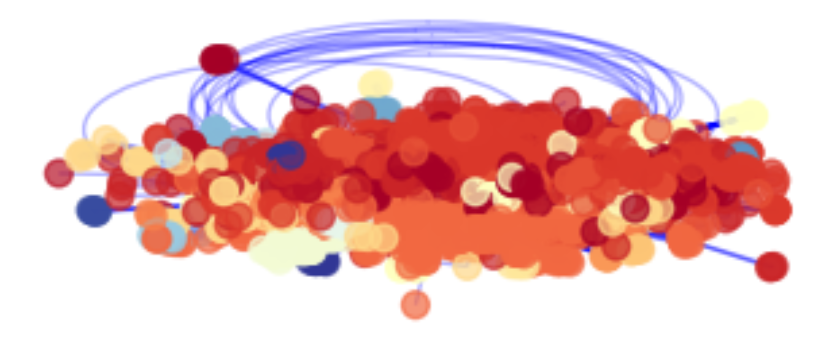
\includegraphics[width=0.5\linewidth]{figures/bcsj_louvain_visualize_part.png}
    \caption{基于louvain算法的社团识别可视化}
    \label{community}
\end{figure}

我们以louvain算法得到的结果(见图\ref{community})为例进行分析:我们无法从可视化中得到较多有用的信息,根据输出结果(见图\ref{compare}),该网络被划分为22个社区,其中比较明显的规律是美国队长、钢铁侠、奇异博士、绯红女巫、蜘蛛侠等超级英雄均被划分为了一组,我们可以推测该组为复仇者联盟;同时,神奇四侠也被划分到了一组。


\begin{figure}[!htbp]
    \centering
    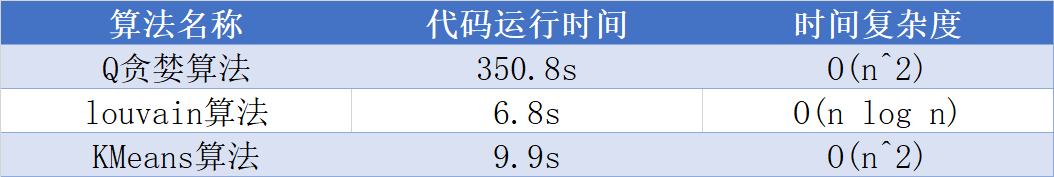
\includegraphics[width=0.8\linewidth]{figures/算法复杂度.jpg}
    \caption{三种算法运算对比}
    \label{compare}
\end{figure}

\subsection{丧尸病毒侵袭——基于网络的传播与动力学}

在漫威宇宙中,丧尸宇宙出现在一个名为《Marvel Zombies》的系列漫画中。这个故事设定了一个被丧尸病毒肆虐的并行宇宙。

在这个丧尸宇宙中,许多超级英雄和反派都被感染成了丧尸,并开始以人类为食。丧尸漫威宇宙的故事情节非常黑暗和血腥,呈现出与正常漫威宇宙相反的景象。该宇宙受到了丧尸病毒的侵袭,随着时间推移,该宇宙中的所有英雄均被感染,并且感染后的英雄利用了穿梭机到达了其他的平行宇宙开始大肆杀戮,现在考虑用SI和SIR模型(假如丧尸病毒解药被研制出,是否可以遏制住病毒的传播?)模拟丧尸病毒在原宇宙中的扩散过程,如图\ref{SISIR}。

\begin{figure}[!htbp]
    \centering
    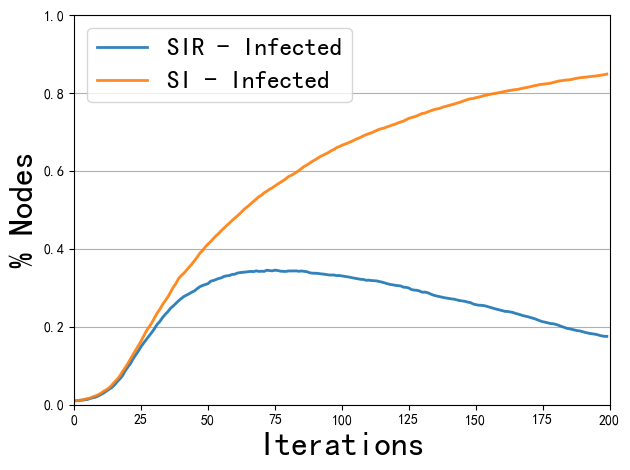
\includegraphics[width=0.5\linewidth]{figures/SI&SIR.png}
    \caption{模拟SI和SIR模型的扩散过程}
    \label{SISIR}
\end{figure}

同时,我们可以应用行为传播模型,模拟当一个邪恶的不好的想法诞生之后,其在英雄网络中的传播情况。

\subsection{总结}

本研究项目旨在探索漫威宇宙中英雄人物之间的关系网络,并研究其拓扑性质,包括节点数、边数、连通片个数、网络聚类系数、平均度和度相关系数等,对漫威宇宙的英雄关系进行了初步的探索。

进一步,本研究结合了五种不同的节点重要性衡量方式,以揭示美国队长是否真正担任着“队长”的角色。经过深入探索,研究结果表明美国队长在该网络中的平均中心度最高,处于核心地位,确实担任着队长的职责。在进一步分析中,本研究还考察了灭霸打响指后网络的情况,并得出结论:若美国队长消失,钢铁侠将成为新的“队长”。

本研究采用了不同种类的节点相似度度量方式,包括基于局部、全局和随机游走的模型,为英雄进行好友推荐。以钢铁侠为例,通过这些模型,为他推荐了最有可能认识的朋友有海妖、黑猫等。

本研究还进行了社团识别的工作,利用三种算法:Q贪婪算法、louvain算法和KMeans算法,对网络进行社团划分,并比较了这三种算法的运行时间和算法核心思路。通过这一步骤,我们能够更好地理解网络中的社团结构和组织关系。

最后,本研究基于网络的传播与动力学分析了丧尸病毒侵袭漫威宇宙的情景,并将其分为有解药和无解药两种情况进行对比。通过研究,我们能够更好地了解丧尸病毒在该宇宙中的传播方式和动力学特征。

综上所述,本研究项目通过对漫威宇宙英雄人物关系网络的探索,研究了其拓扑性质、节点重要性、节点相似度、社团识别以及传播与动力学等方面的内容,为理解该宇宙中角色关系和事件影响提供了深入的分析。这些研究结果对进一步探索漫威宇宙及其他复杂网络系统具有重要的参考价值。

\section{基于三体世界的文本分析}

\subsection{介绍}

《三体》是刘慈欣创作的一部科幻小说三部曲,包括《三体》、《黑暗森林》和《死神永生》。这个系列小说以宇宙间的对抗和人类文明的命运为主题,融合了科学、哲学和文化等多个领域的元素,被誉为中国科幻文学的经典之作。

故事背景设定在近未来的中国,地球面临着威胁和危机。一批科学家发现了一个名为“三体”的外星文明,并向其发送了地球的信号。然而,三体文明的世界“三体”恶劣的环境和不稳定的星系轨道使他们对外界持悲观态度,决定入侵地球。

小说通过多个角色的视角,描绘了人类社会对抗三体文明的过程。其中包括一名年轻的女物理学家叶文洁、一位叫做罗辑的天才数学家以及一批秘密组织与政府力量。故事在科幻的框架下涉及了众多的科学概念和哲学思考,包括虚拟现实、宇宙物理学、人工智能等等。

《三体》系列小说以其宏大的背景和深刻的思考而受到广泛关注和赞誉。它引人入胜的情节、复杂的人物关系和深刻的哲学探索使其成为一部富有想象力和独特视角的科幻作品。该系列小说荣获了多个奖项,包括雨果奖(Hugo Awards)等国际科幻文学奖项,也为中国科幻文学在国际上赢得了广泛的认可。


\subsection{分词及词云可视化}

\pagestyle{fancy}
\fancyhf{} % 清空当前的页眉页脚设置
\renewcommand{\headrulewidth}{0pt} % 设置页眉下划线宽度为 0
\lhead{\itshape 基于三体世界的文本分析}
\rhead{\thepage}

我们从网上获取了《三体》三部曲的txt文档,部分节选如下图\ref{content_threebody}。

\begin{figure}[!htbp]
    \centering
    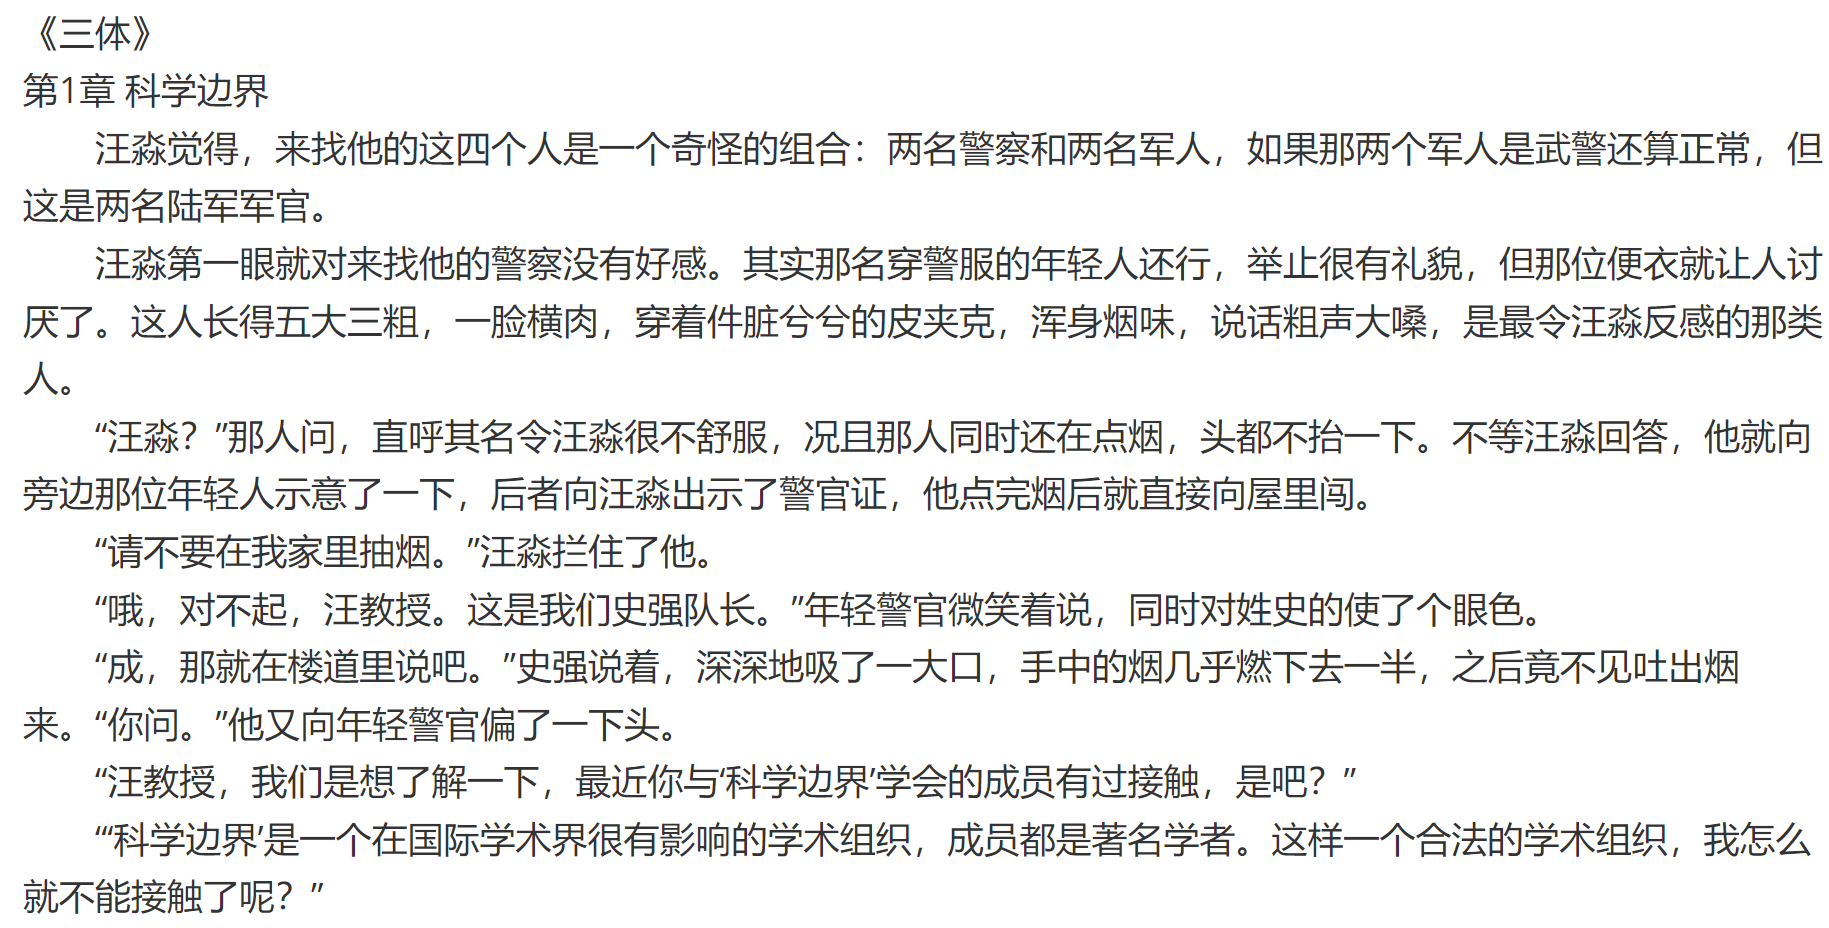
\includegraphics[width=\linewidth]{figures/三体部分节选.png}
    \caption{三体部分节选}
    \label{content_threebody}
\end{figure}

我们利用jieba分词库对《三体》内容进行分词、停用词过滤,根据出现的频次进行了统计,我们利用wordCloud绘制词云,轮廓为三体舰队中水滴的模型,如图\ref{content_wordcloud_count}。

\begin{figure}[htbp]
    \centering
    \begin{subfigure}[b]{0.5\textwidth}
        \centering
        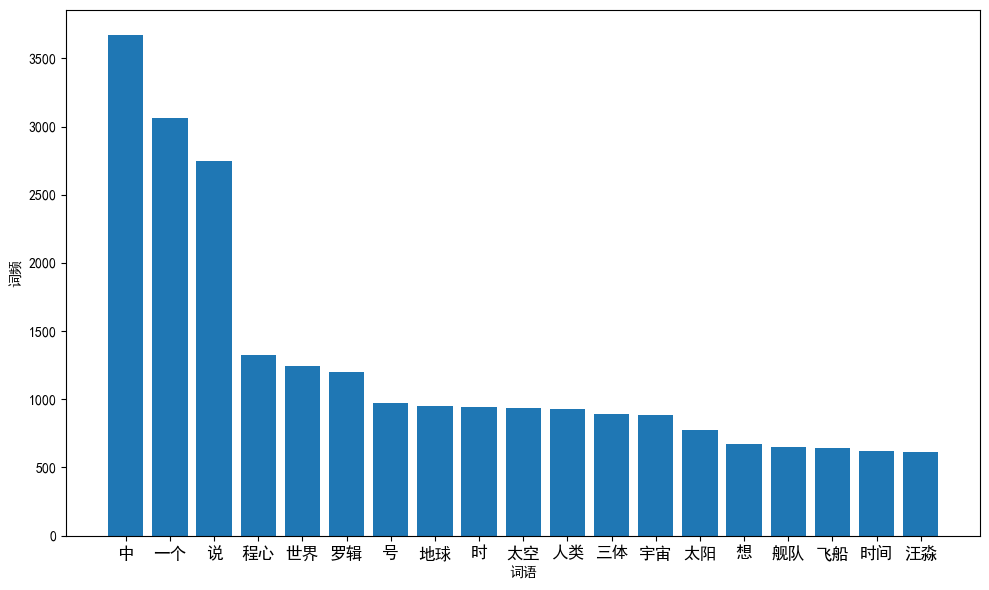
\includegraphics[width=\linewidth]{figures/词频统计.png}
        \caption{词频统计}
        \label{content_count}
        \end{subfigure}
    \hspace{0.05\textwidth} % 调整两张图片之间的间距
    \begin{subfigure}[b]{0.4\textwidth}
        \centering
        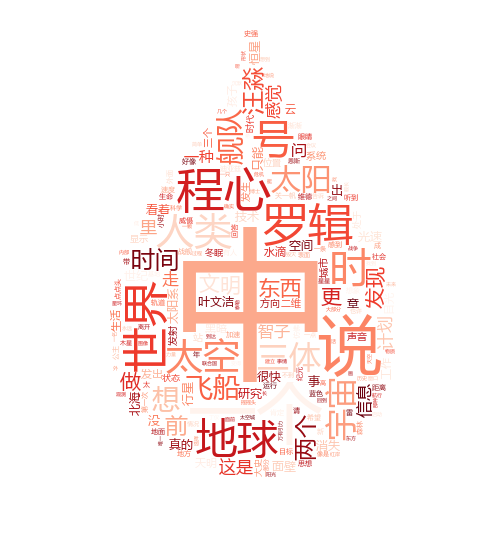
\includegraphics[width=\textwidth]{figures/三体词云.png}
        \caption{三体词云}
        \label{content_wordcloud}
    \end{subfigure}
    \caption{词频词云可视化}
    \label{content_wordcloud_count}
  \end{figure}

\subsection{基于不同表示方法的词语相似度度量}
由于《黑暗森林》和《死神永生》章节划分较为模糊,我们仅选取《三体》第一部进行探索。在进行不同词的不同表示方法前,我们需要对数据进行一些预处理,包括:读取txt文件、分词、按照章节汇总。

\subsubsection{基于词袋模型的相似度指标}
针对词袋模型, D2M矩阵(Document-Term Matrix)表示文档和词语之间的关系,每一列代表一个词语的频率或计数。如果你希望计算某个词语与其他词语之间的相似度,可以将该词语的列视为一个向量,并使用余弦相似度计算与其他词语列向量的相似度。

下面是一种基本的计算方法:

1.	首先,从D2M矩阵中选择某个词语的列,将其作为向量A。

2.	对于其他词语的列向量,分别将它们作为向量B。

3.	使用余弦相似度公式计算向量A与向量B之间的相似度,得到一个相似度值。

4.	重复步骤2和步骤3,计算向量A与其他所有词语的相似度。

这样,你可以获得词语与其他词语之间的相似度度量,其中相似度值越接近1表示词语越相似,值越接近0表示词语越不相似。

需要注意的是,词袋模型是基于词语频率或计数的表示方法,忽略了词语的顺序和语义关系。因此,通过词袋模型计算的词语相似度主要是基于词语在不同文档中的共现情况进行的,不能完全捕捉词语的语义相似性。对于更准确的词语相似度计算,通常需要使用词嵌入模型(如Word2Vec、GloVe等)来获得词语的分布式表示,并计算词向量之间的相似度。

下面我们分别以叶文洁、三体、汪淼、丁仪为例,计算于其最详尽的五个词语排名,结果如图\ref{combine2}

\begin{figure}[t]
    \centering
    \begin{subfigure}[b]{0.4\textwidth}
        \centering
        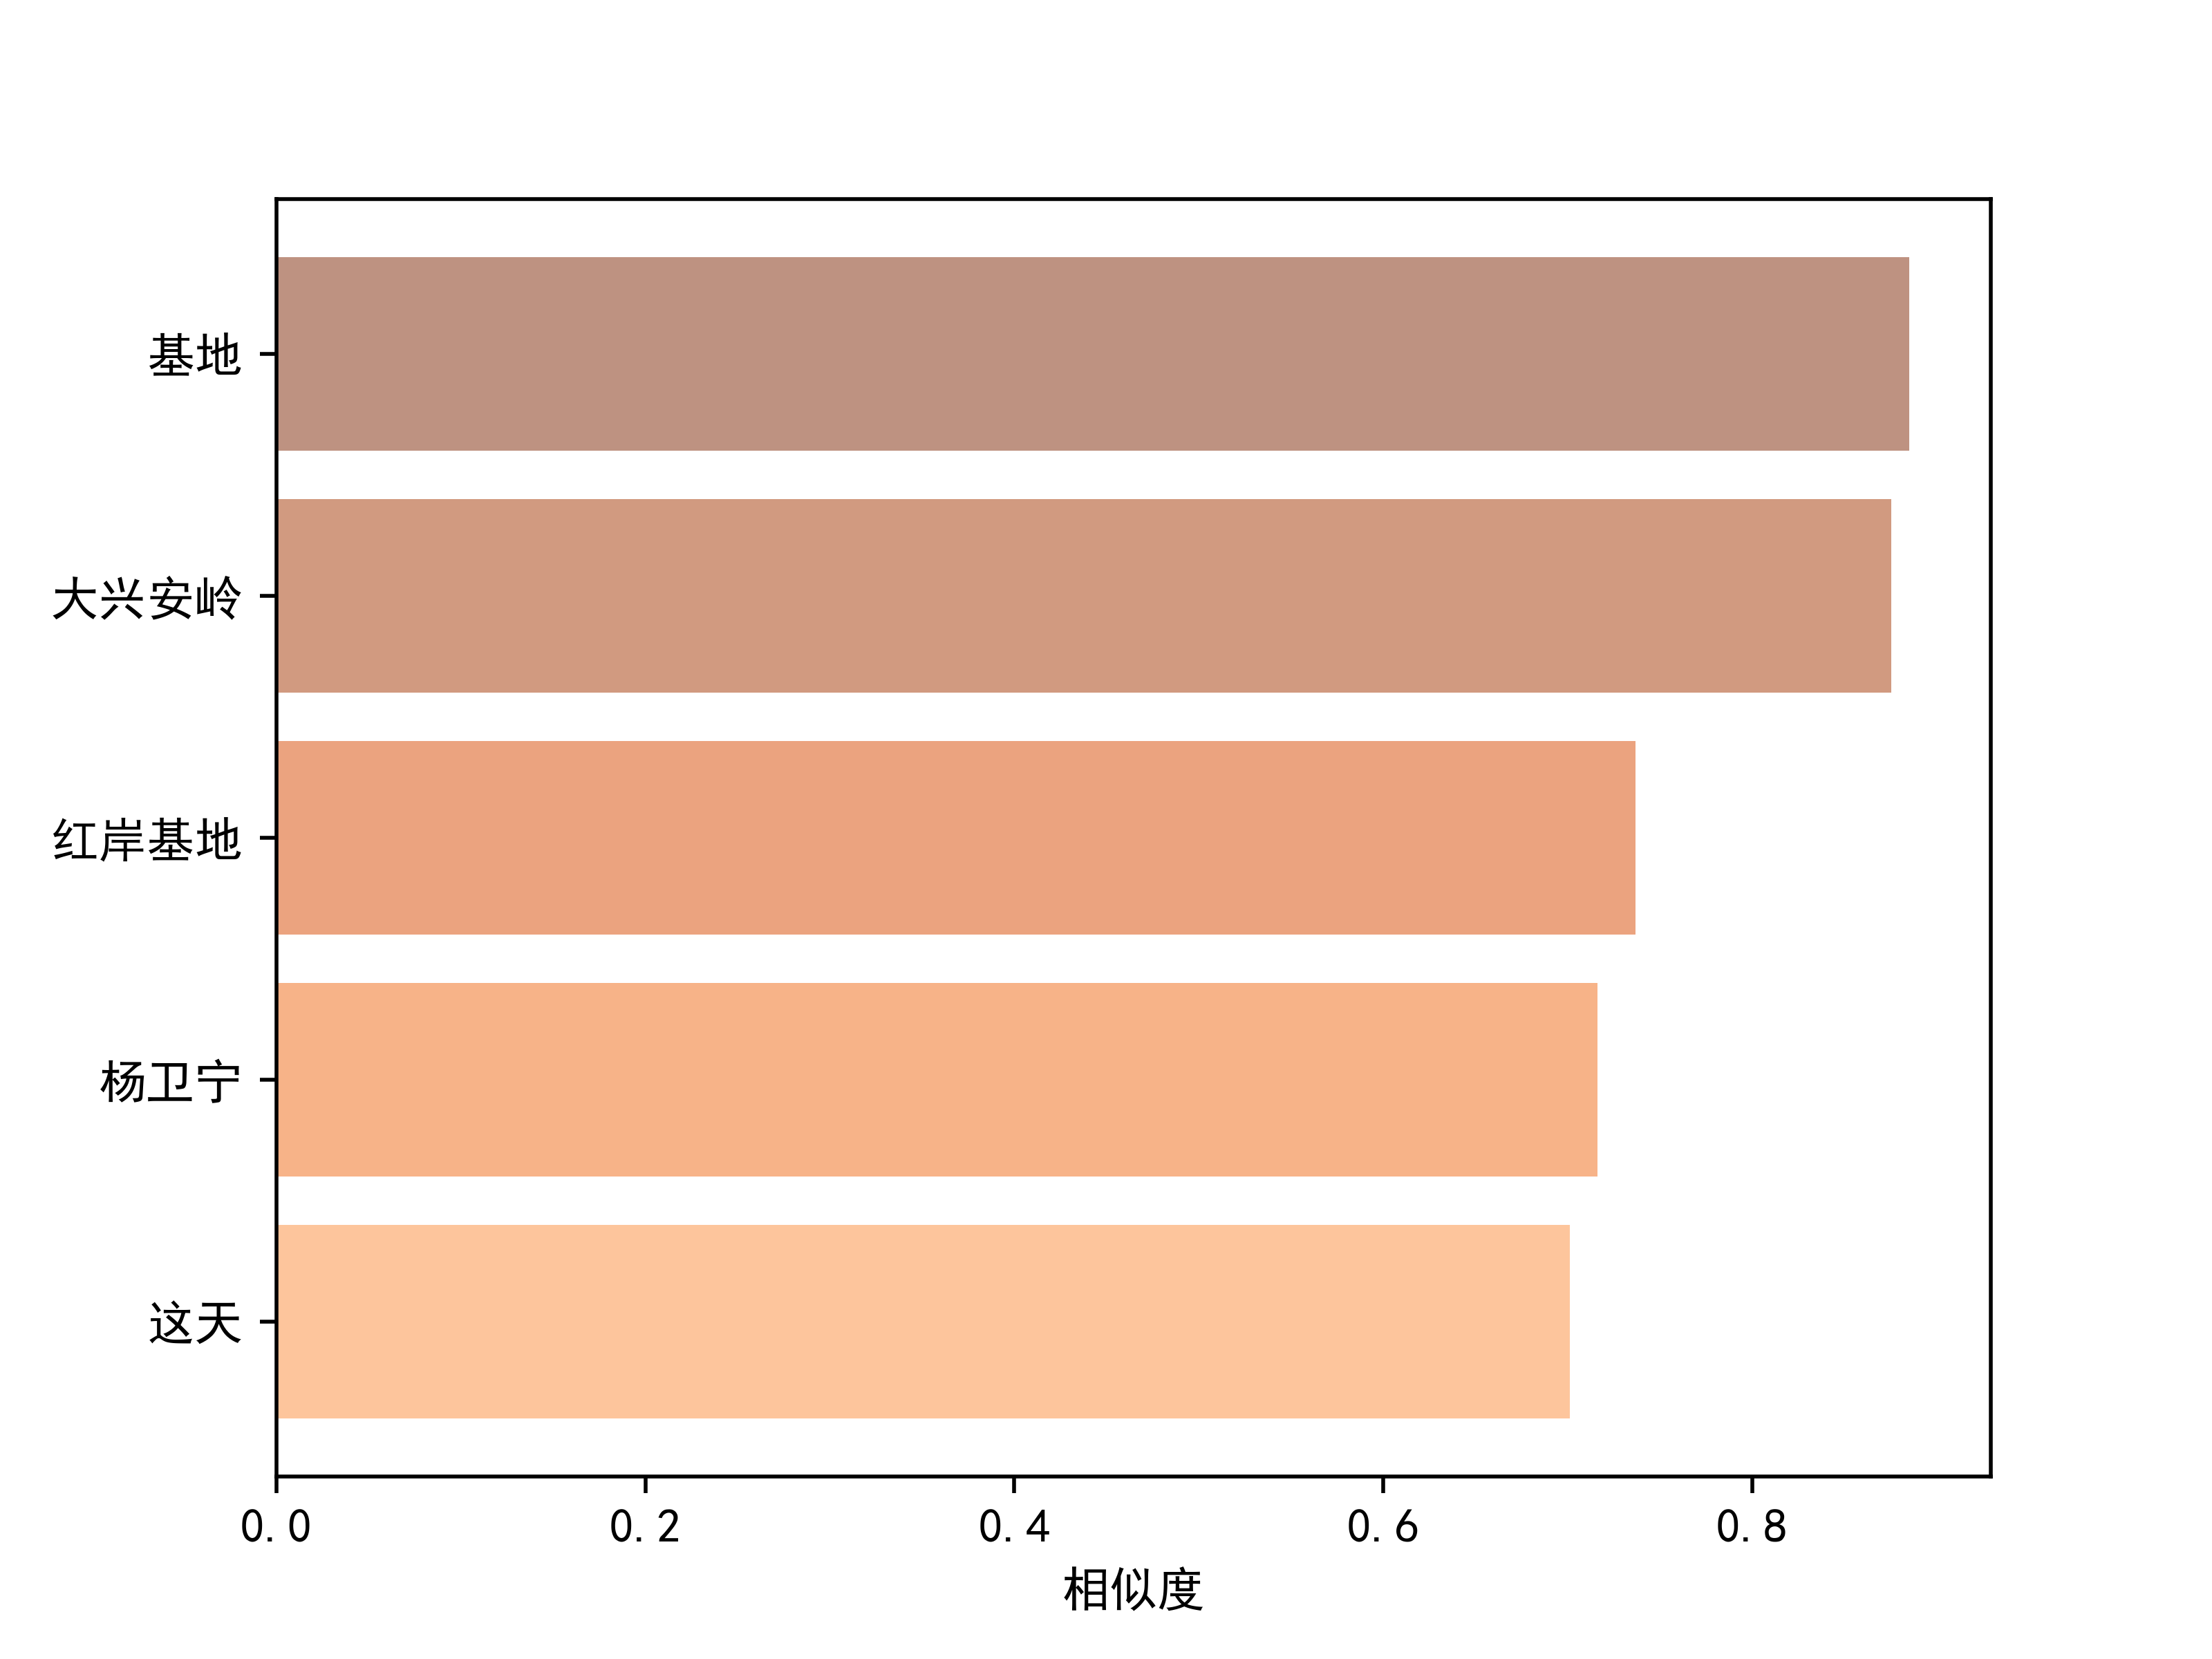
\includegraphics[width=\linewidth]{figures/叶文洁词袋模型.png}
        \caption{与叶文洁相似的词语前五名}
        \label{yewenjie}
        \end{subfigure}
    \hspace{0.05\textwidth} 
    \begin{subfigure}[b]{0.4\textwidth}
        \centering
        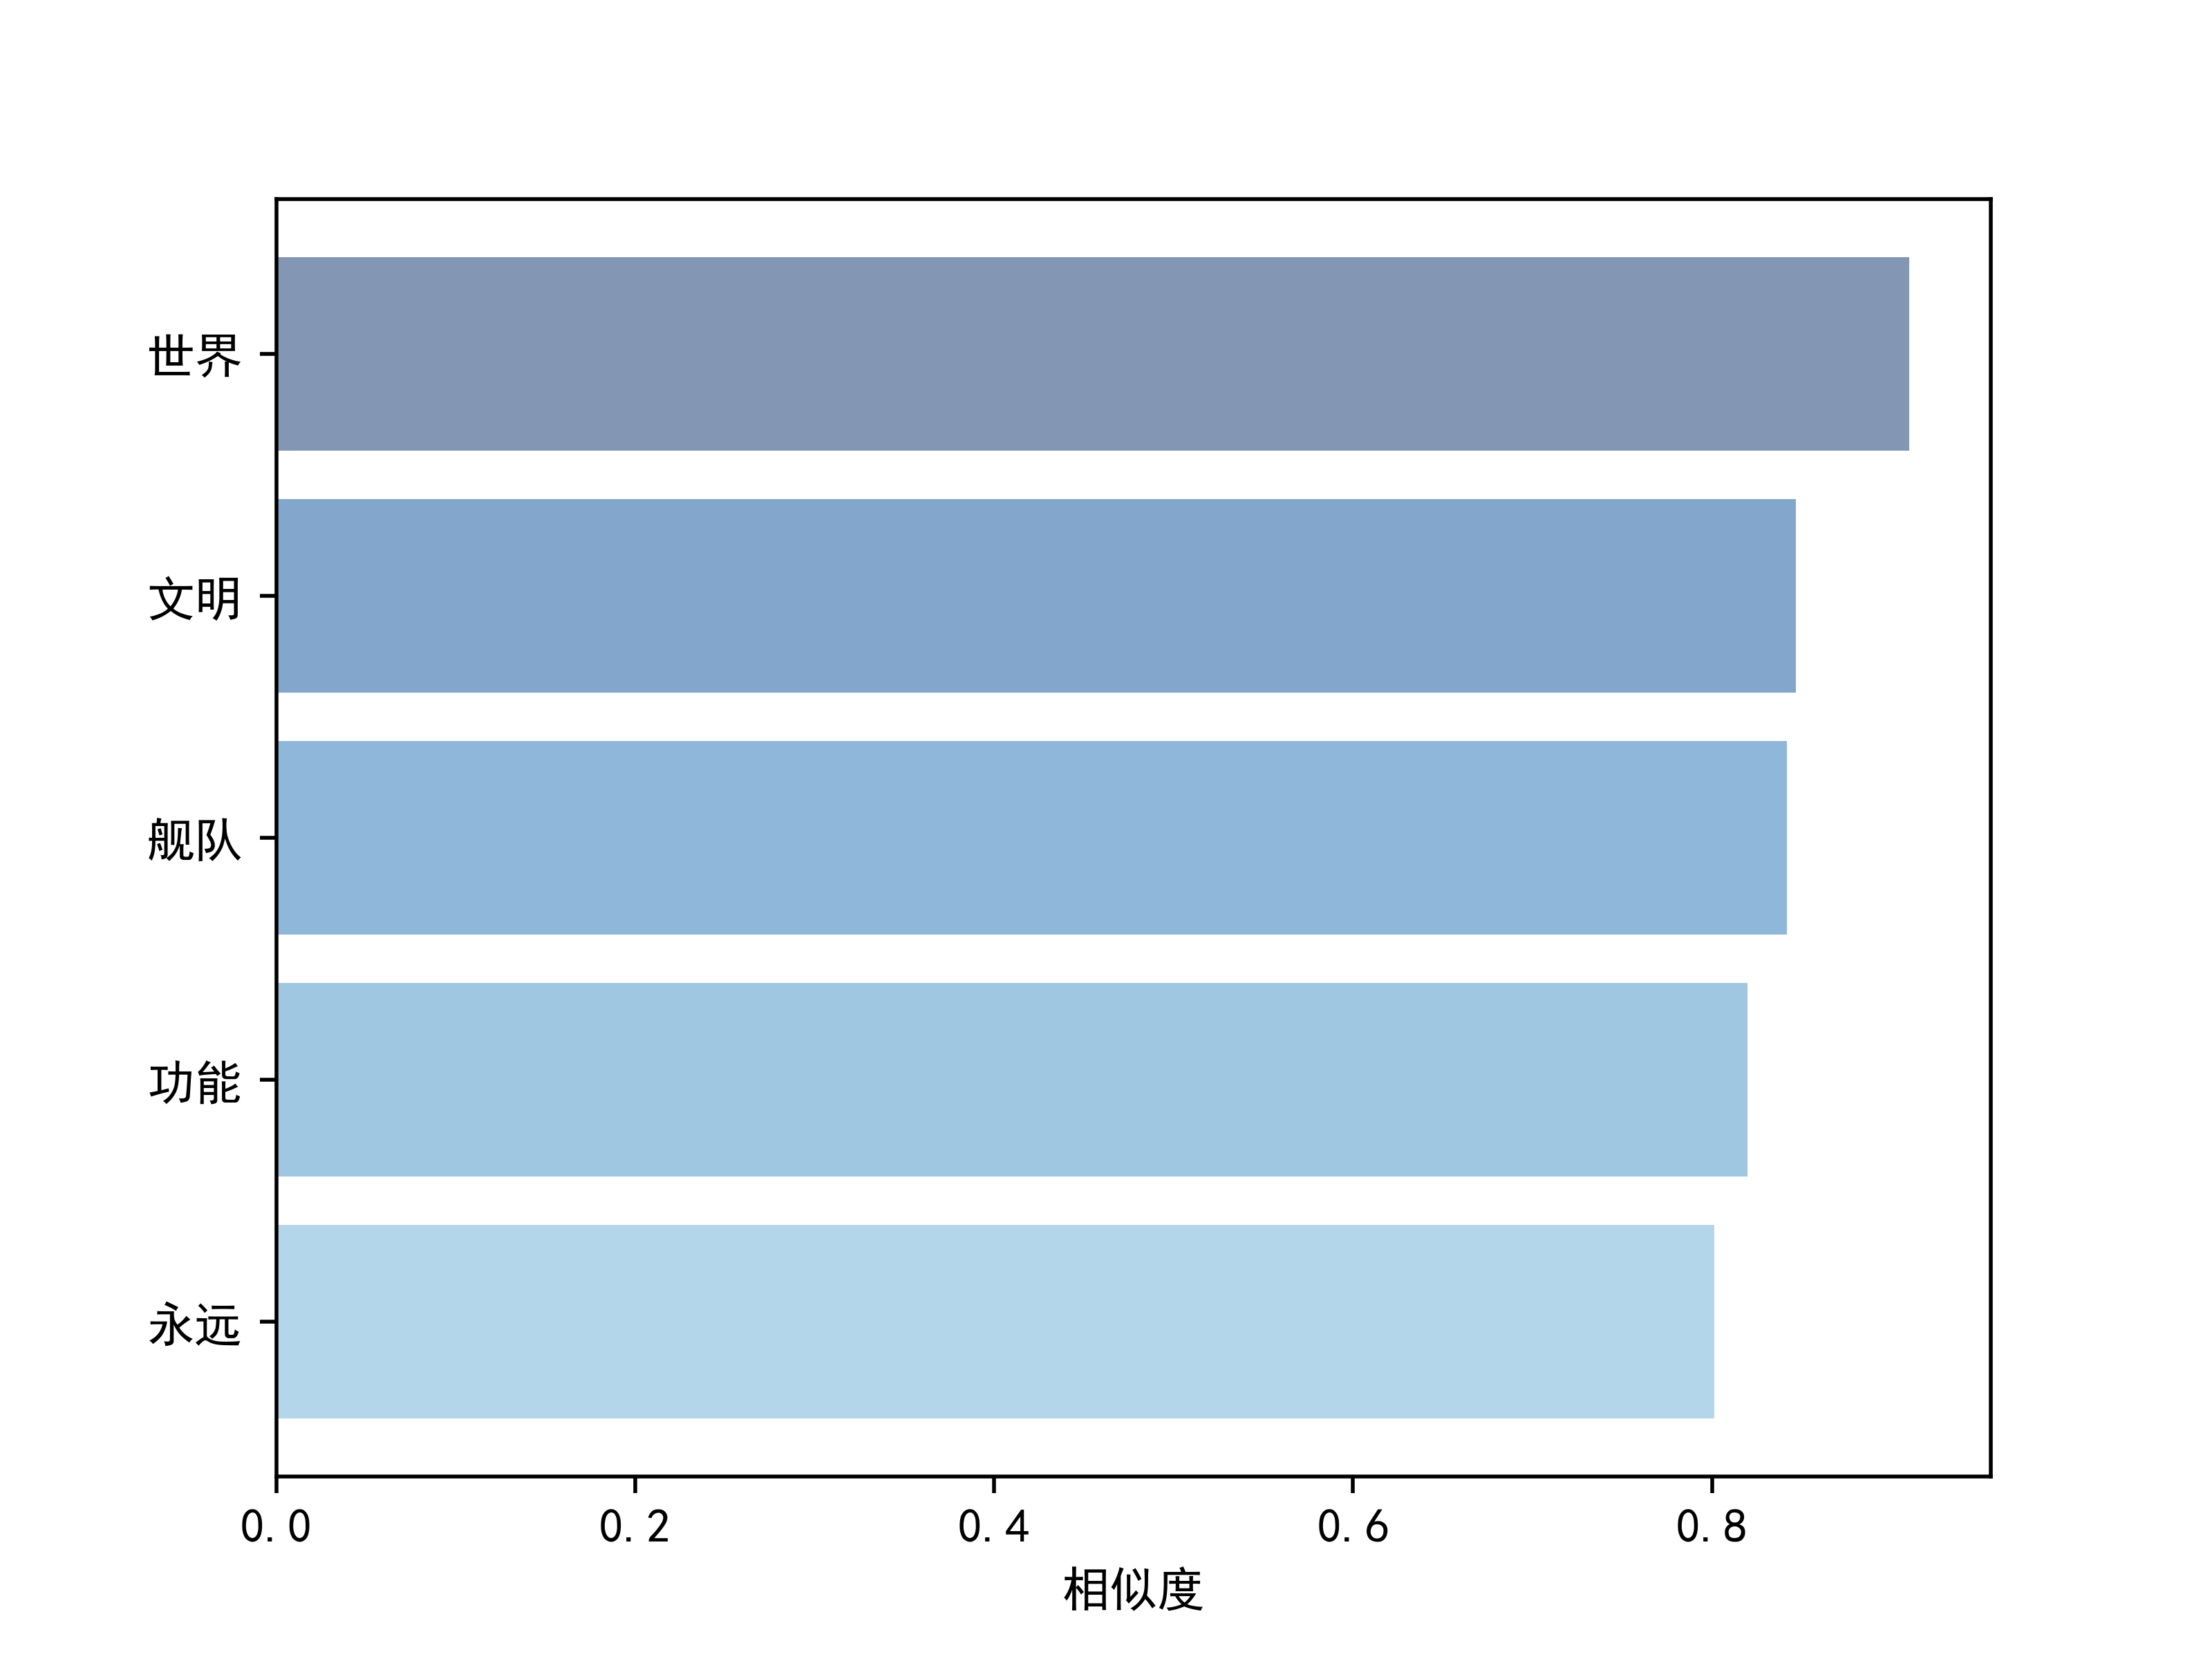
\includegraphics[width=\textwidth]{figures/三体词袋模型.png}
        \caption{与三体相似的词语前五名}
        \label{santi}
    \end{subfigure}
    \label{combine1}
  \end{figure}

\begin{figure}[t]
    \centering
    \begin{subfigure}[b]{0.4\textwidth}
        \centering
        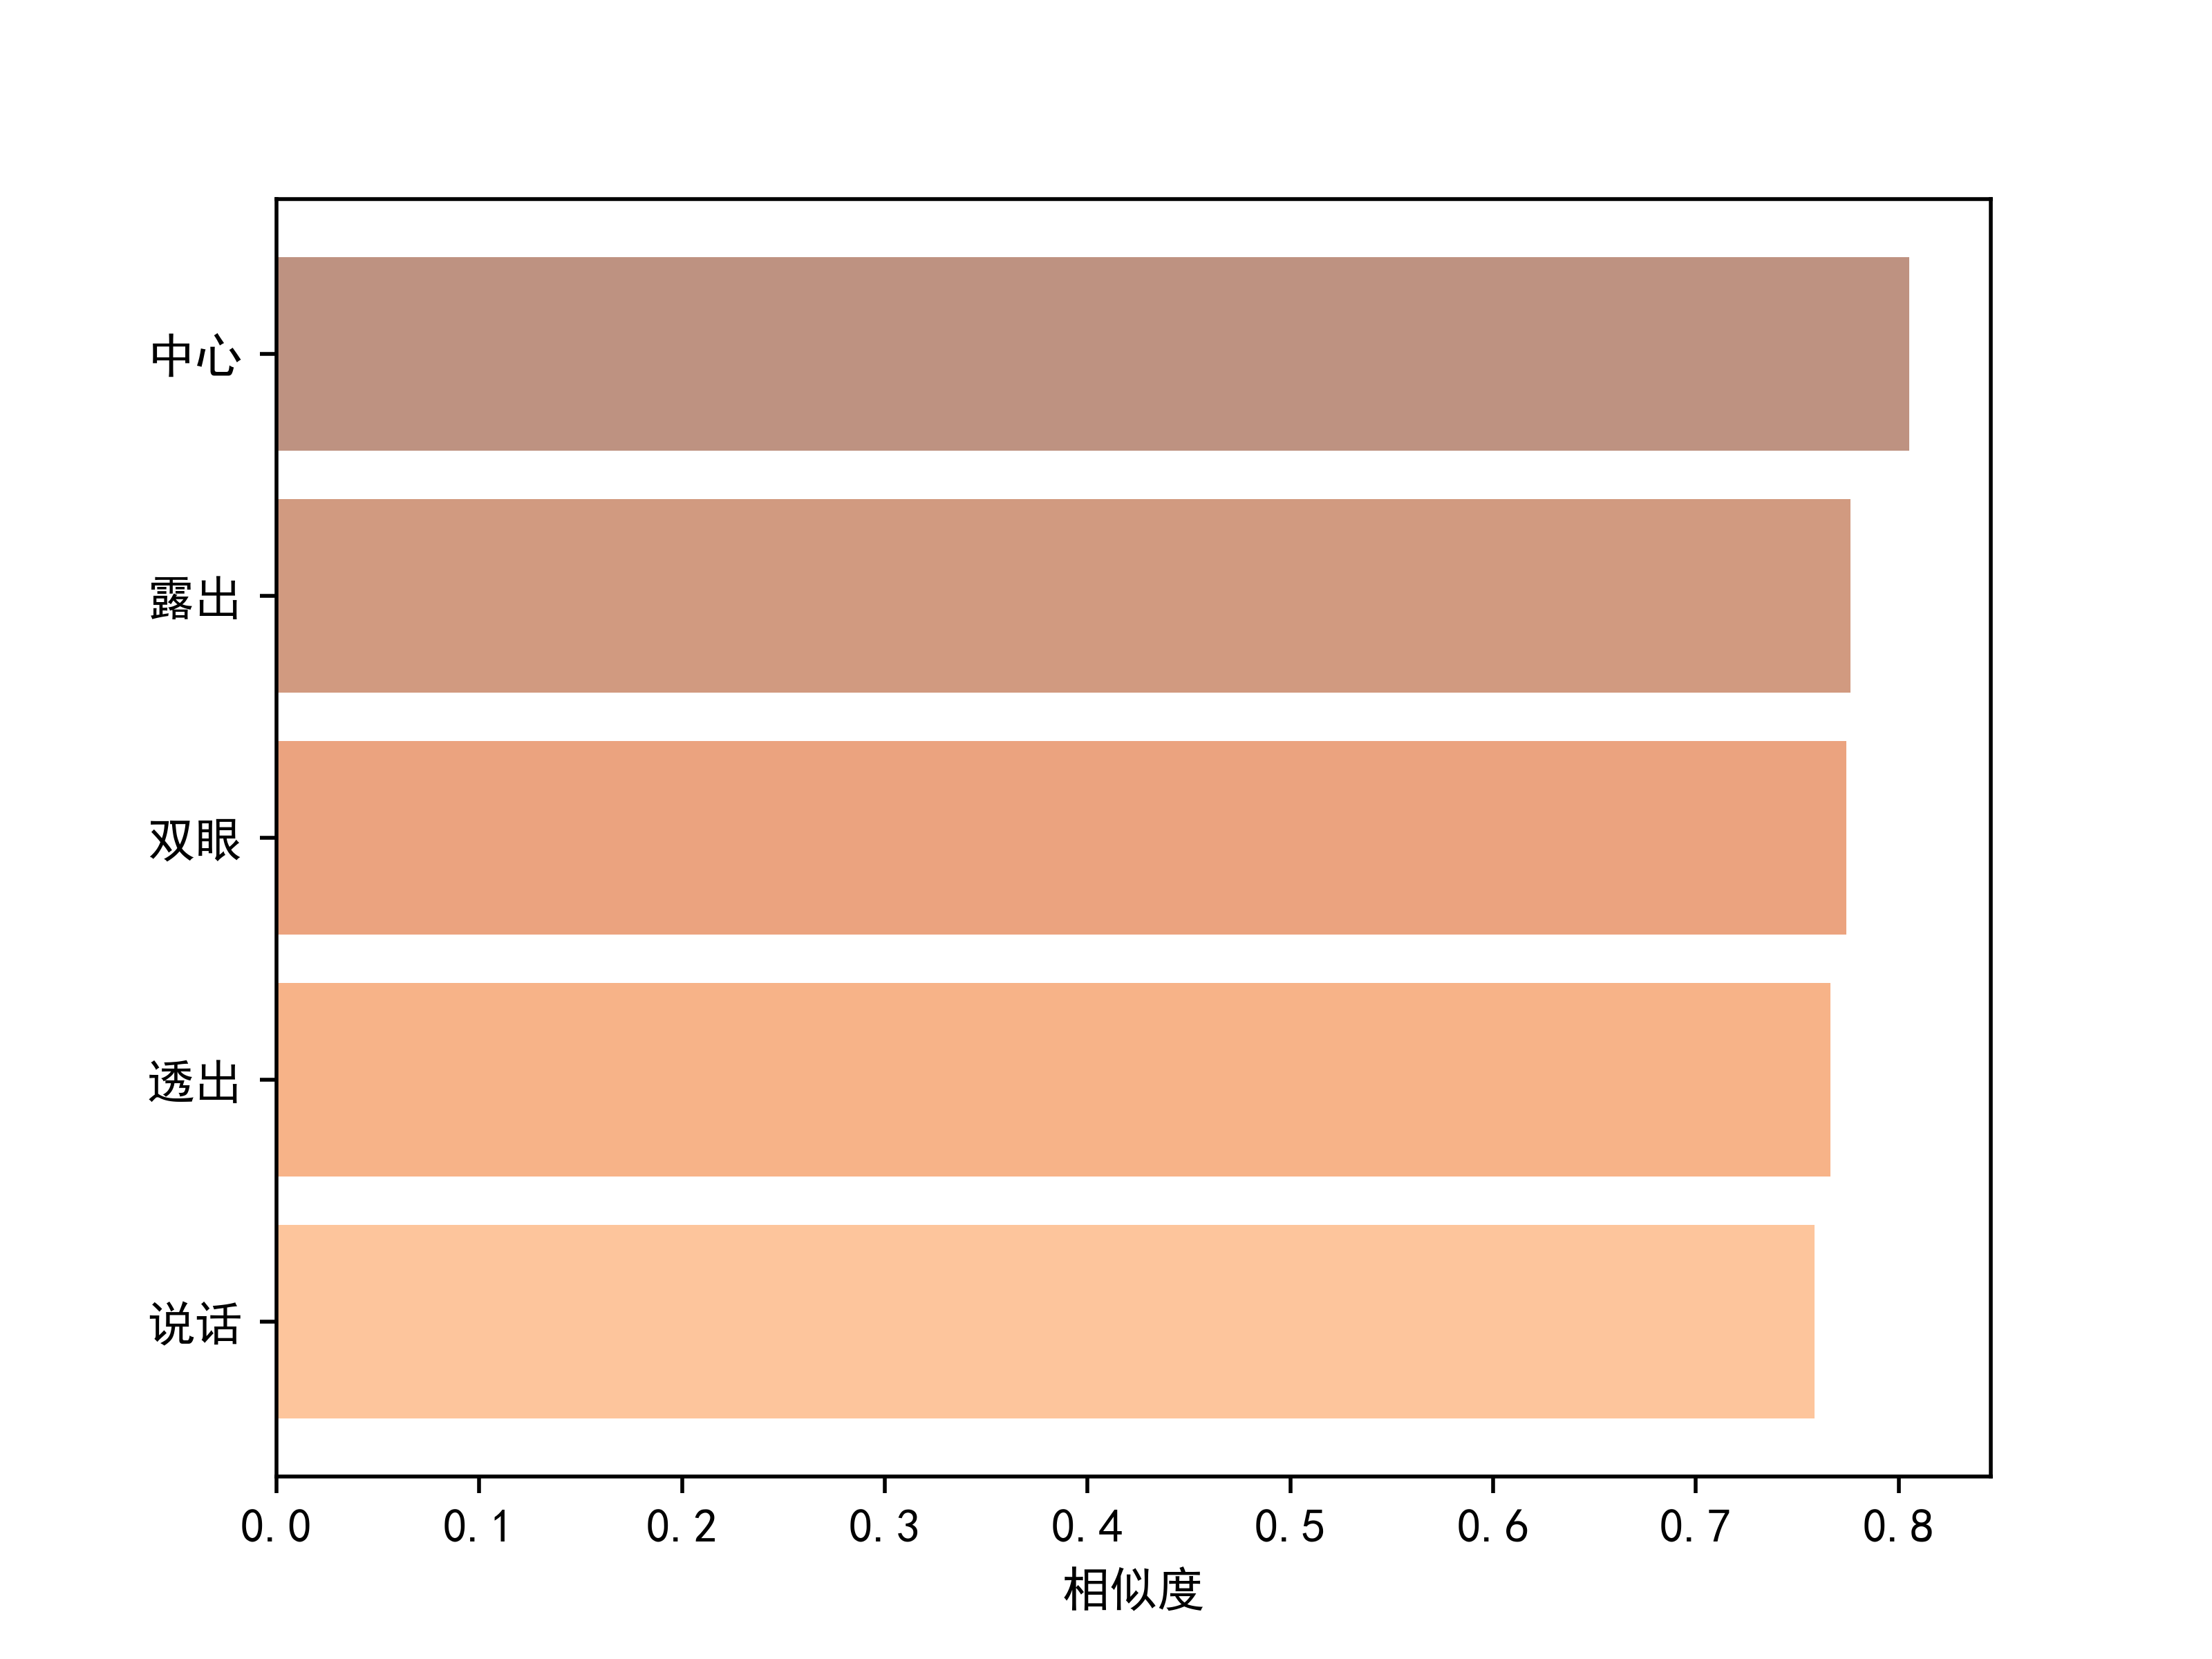
\includegraphics[width=\linewidth]{figures/汪淼词袋模型.png}
        \caption{与汪淼相似的词语前五名}
        \label{wangmiao}
        \end{subfigure}
    \hspace{0.05\textwidth} % 调整两张图片之间的间距
    \begin{subfigure}[b]{0.4\textwidth}
        \centering
        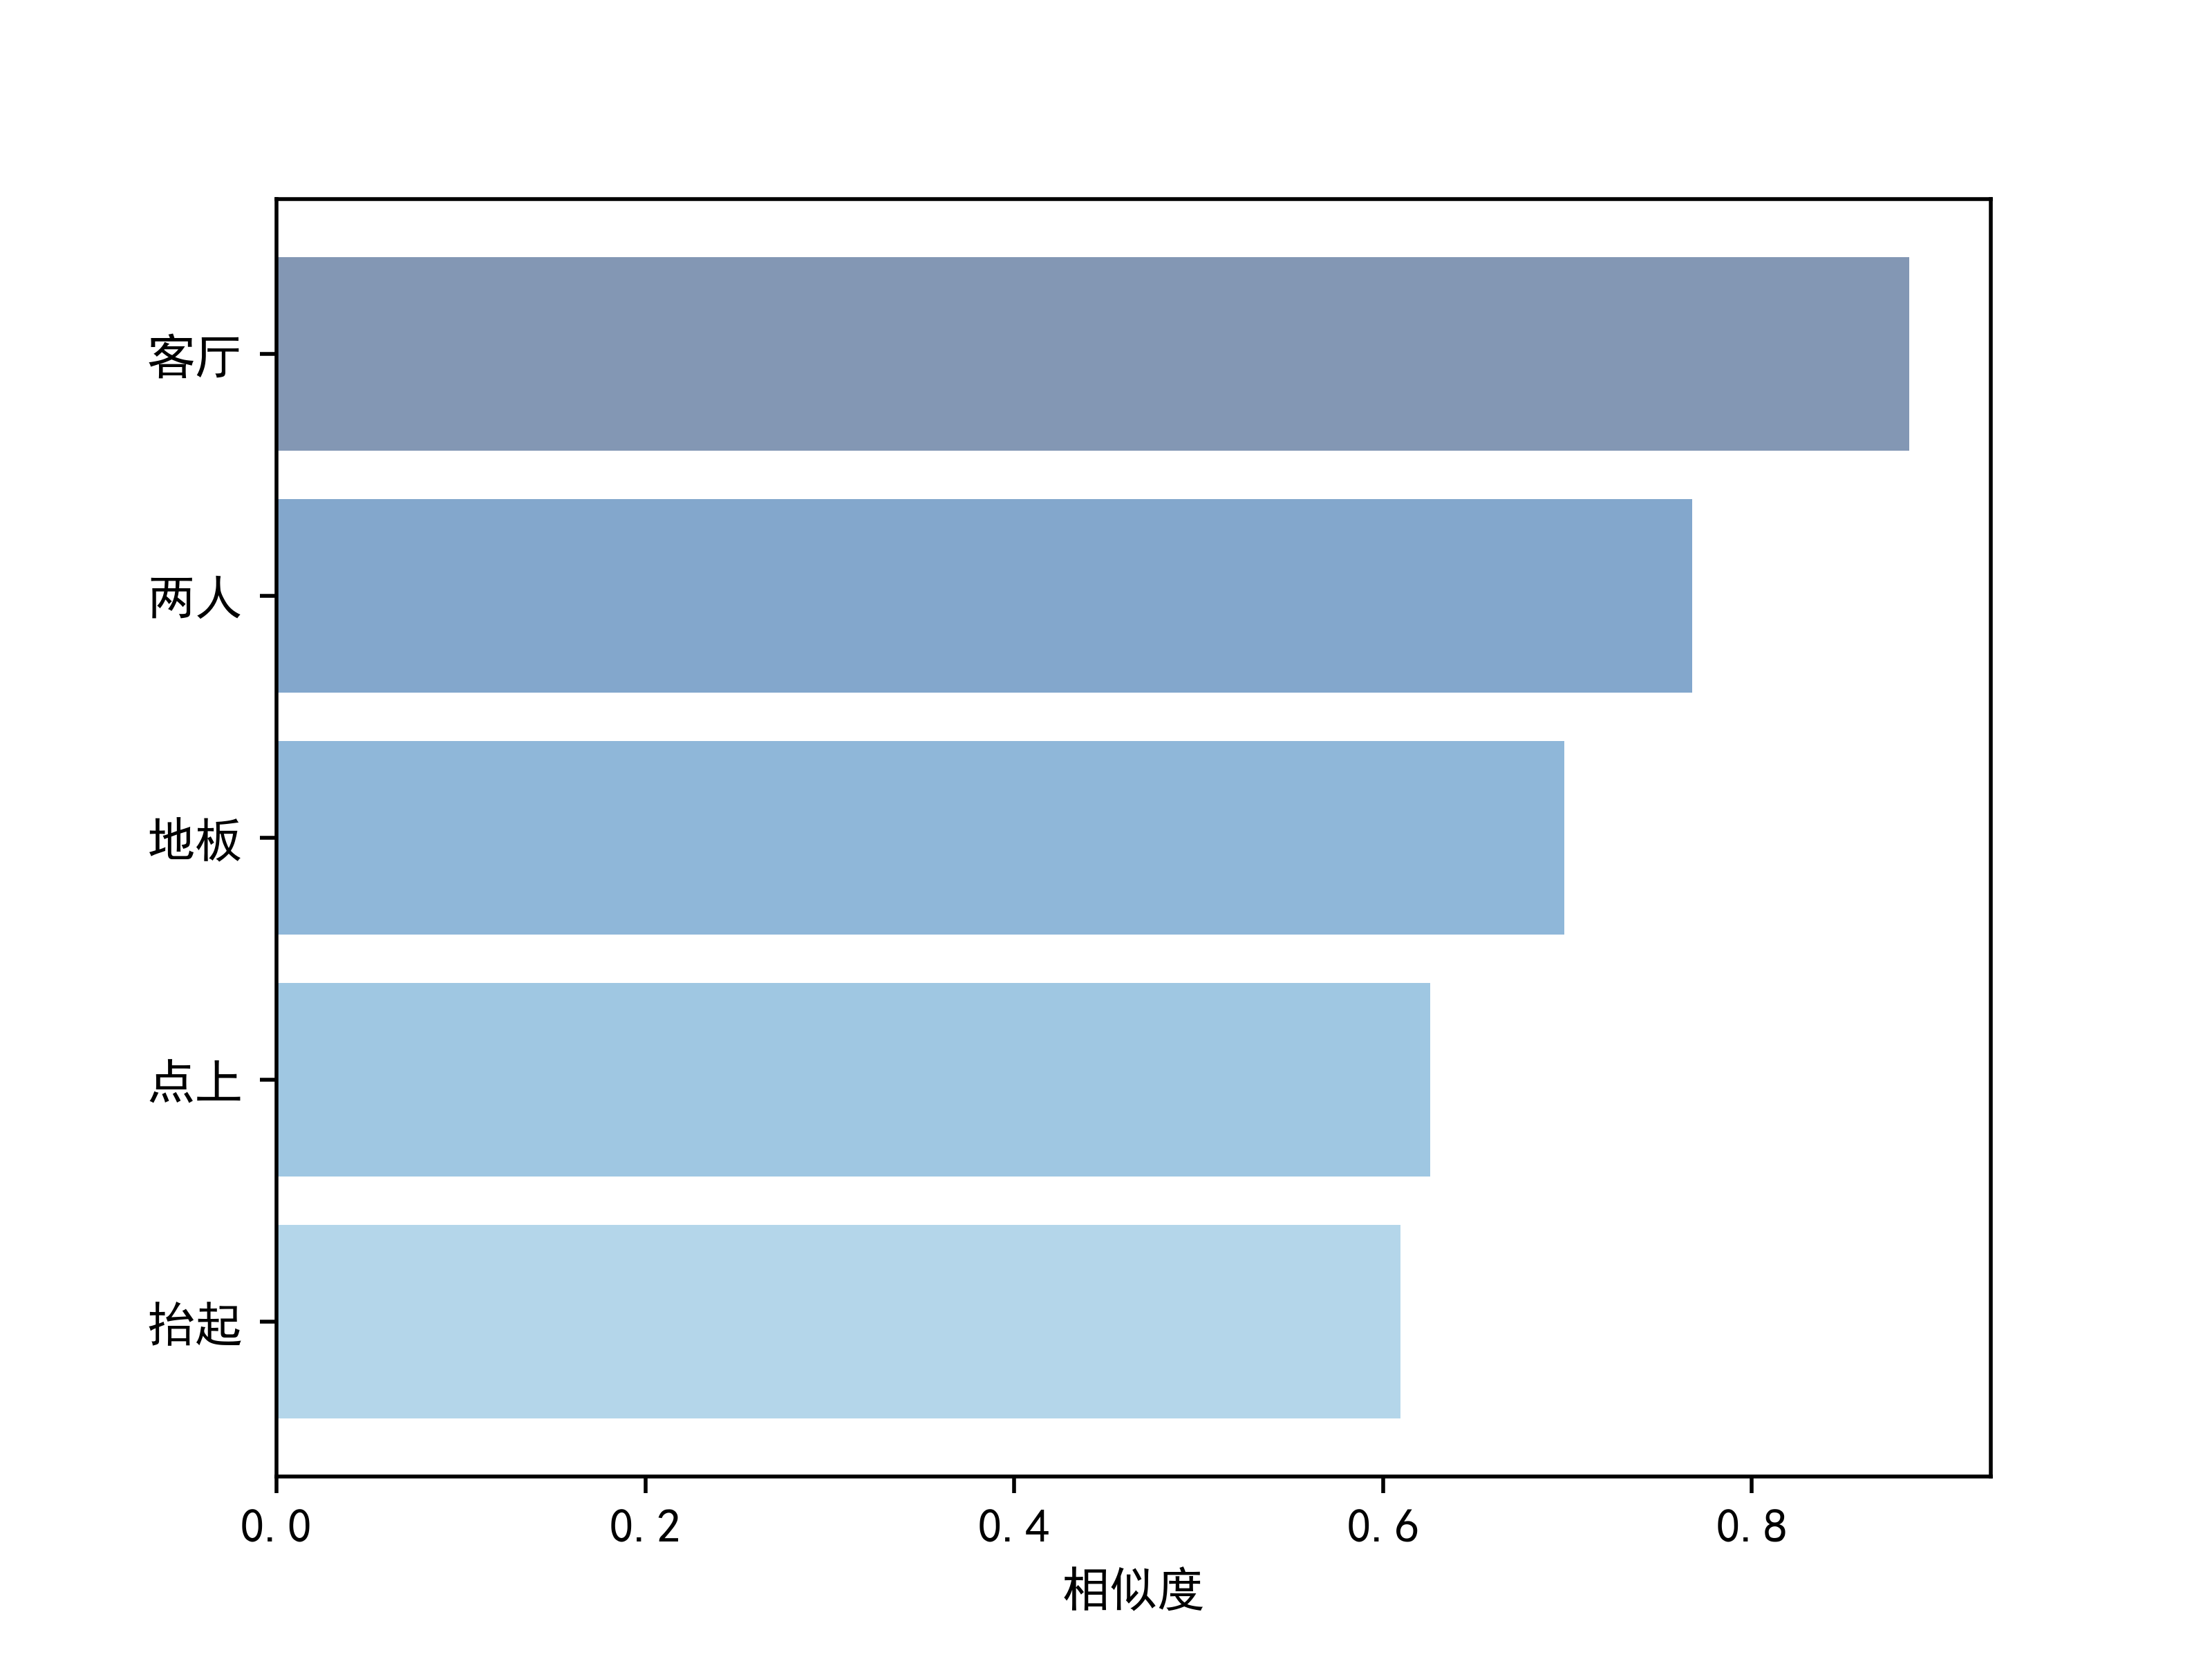
\includegraphics[width=\textwidth]{figures/丁仪词袋模型.png}
        \caption{与丁仪相似的词语前五名}
        \label{dingyi}
    \end{subfigure}
    \caption{基于词袋模型词语相似度排名}
    \label{combine2}
\end{figure}

相似度结果计算如下:与叶文洁相似的词语前五名分别为\textbf{基地、大兴安岭、红岸基地、杨卫宁、这天};与三体相似的词语前五名分别为\textbf{世界、文明、舰队、功能、永远};与汪淼相似的词语前五名分别为\textbf{中心、露出、双眼、透出、说话};与丁仪相似的词语前五名分别为\textbf{客厅、两人、地板、点上、抬起}。

\subsubsection{基于Bi-gram模型的相似度指标}

针对Bi-gram模型,n-gram模型是一种基于统计的文本模型,它将文本切分为固定长度的连续序列,称为n-gram。每个n-gram被视为一个独立的单元,忽略了词语的顺序和语义关系。由于n-gram模型仅考虑文本中的局部上下文,而无法捕捉到整体语义信息,我们假设两个单词越临近,则其相关程度越大,相似度越高。 

下面我们同样以叶文洁、三体、汪淼、丁仪为例,计算于其最详尽的五个词语排名,如图\ref{Bi-gram}。

\begin{figure}[!htbp]
    \centering
    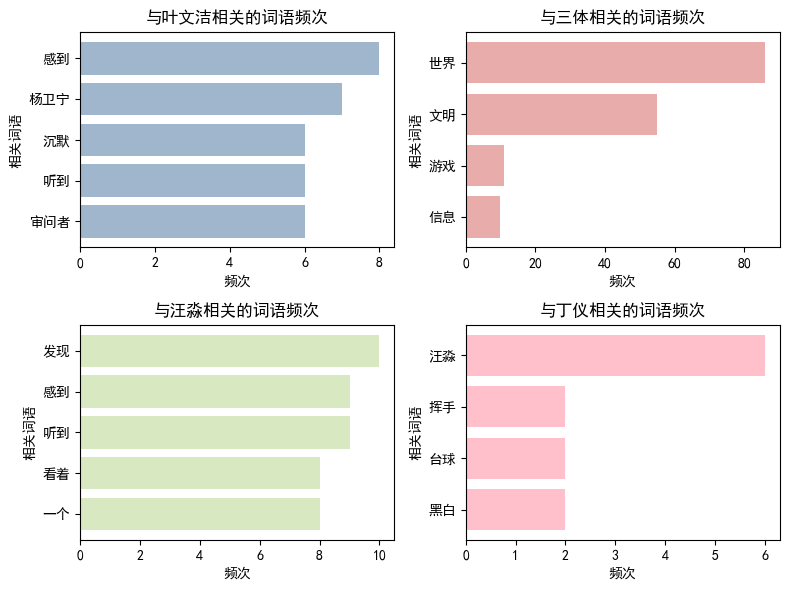
\includegraphics[width=0.8\linewidth]{figures/Bi-gram.png}
    \caption{基于Bi-gram模型词语相似度排名}
    \label{Bi-gram}
\end{figure}

相似度结果计算如下:与叶文洁相似的词语前五名分别为\textbf{感到、杨卫宁、沉默、听到、审问者};与三体相似的词语前四名(有一个重复了)分别为\textbf{世界、文明、游戏、信息};与汪淼相似的词语前五名分别为\textbf{发现、感到、听到、看看、一个};与丁仪相似的词语前四名分别为\textbf{汪淼、挥手、台球、黑白}。

\subsubsection{基于Word2Vec的相似度指标}

针对 Word2Vec 模型,Word2Vec 是一种基于神经网络的词嵌入模型,它通过训练将词
语映射到一个连续的低维向量空间中。Word2Vec 的核心思想是通过预测上下文或目标词语
来学习词语的分布式表示,即词向量。Word2Vec 模型在训练过程中,通过分析大量的文本
数据,尝试捕捉词语之间的语义和语法关系。在生成词向量时,相似的词语在向量空间中会
有较近的距离,这使得我们可以使用向量之间的距离或相似度来衡量词语之间的相似性。

\begin{figure}[!htbp]
    \centering
    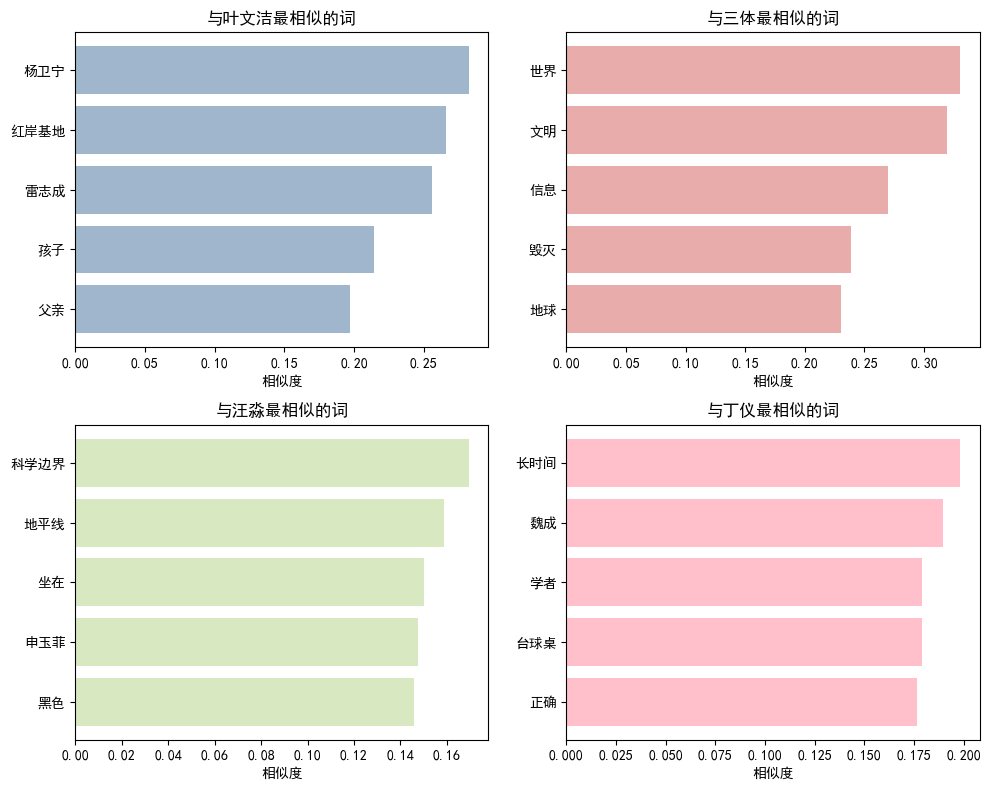
\includegraphics[width=0.8\linewidth]{figures/word2vec.png}
    \caption{基于word2vec模型词语相似度排名}
    \label{word2vec}
\end{figure}

相似度结果计算如下:与叶文洁相似的词语前五名分别为\textbf{杨卫宁、红岸基地、雷志成、孩子、父亲};与三体相似的词语前五名分别为\textbf{世界、文明、信息、毁灭、地球};与汪淼相似的词语前五名分别为\textbf{科学边界、地平线、坐在、申玉菲、黑色};与丁仪相似的词语前五名分别为\textbf{长时间、魏成、学者、台球桌、正确}。

\subsubsection{三种词的表示方法的比较及应用场景}

\textbf{词袋模型:}

1.	特点:将文本表示为离散的词袋,完全没有利用语序信息,忽略了词语的顺序和语义关系,仅考虑词语的频率。

2.	应用场景:适用于文本分类、情感分析、关键词提取等任务,尤其在对文本整体特征不敏感的场景中效果较好。

\textbf{Bi-gram模型:}

1.	特点:将文本切分为固定长度的连续序列,考虑局部上下文信息,忽略了词语的顺序和语义关系。同时当词数量提升,词表迅速膨胀,数据出现大量稀疏化问题。

2.	应用场景:适用于语言建模、文本生成和文本分类等任务,尤其在考虑相邻词语间关系的局部特征时有一定效果。

\textbf{Word2Vec模型:}

1.	特点:基于神经网络,通过训练将词语映射到连续的低维向量空间中,捕捉词语之间的语义关系。

2.	应用场景:适用于词语相似度计算、词语聚类、文本分类、命名实体识别等任务,尤其在需要考虑词语的语义特征和语义关系时表现较好。

\subsection{关键词提取与主题识别}

关键词提取算法主要有两类:无监督关键词提取方法和有监督关键词提取方法。

无监督关键词提取方法不需要人工标注的语料,利用某些方法发现文本中比较重要的词作为关键词,进行关键词提取。该方法是先抽取出候选词,然后对各个候选词进行打分,然后输出topK个分值最高的候选词作为关键词。根据打分的策略不同,有不同的算法,例如基于统计特征的TF-IDF算法,基于词图模型的TextRank,基于主题模型的LDA等算法。

有监督关键词提取方法将关键词抽取过程视为二分类问题,先提取出候选词,然后对于每个候选词划定标签,要么是关键词,要么不是关键词,然后训练关键词抽取分类器。当新来一篇文档时,提取出所有的候选词,然后利用训练好的关键词提取分类器,对各个候选词进行分类,最终将标签为关键词的候选词作为关键词。

下面以三体第一章节为例,利用无监督关键词提取方法中的TF-IDF算法,提取的关键词如下图\ref{TF-IDF}(仅展示前五章)

\begin{figure}[!htbp]
    \centering
    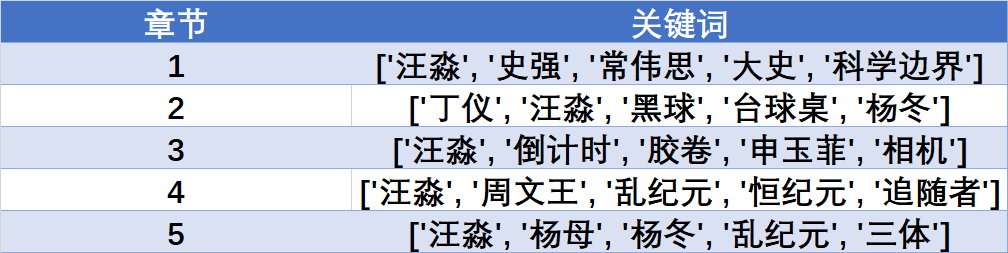
\includegraphics[width=0.8\linewidth]{figures/TF-IDF关键词.jpg}
    \caption{基于TF-IDF模型的关键词提取}
    \label{TF-IDF}
\end{figure}

\subsection{文档的相似性与应用}

\subsubsection{文本相似度}

文档的相似度有如下三种常用计算方法:

\begin{enumerate}
    \item 基于词袋模型的相似度计算:
    
    词频相似度:两个文本的用词越接近,他们的内容相似度越高。

    \item 基于Word2vec的文档相似度:
    
    word2vec取平均:较短的文档如果希望计算文本相似度,可以将各自内部的word2vec向量分别进行平均,用平均后的向量作为文本向量,从而用于计算相似度。

    \item 基于doc2vec的文档相似度:
    
    doc2vec是word2vec的拓展,它可以直接获得sentences/paragraphs/documents的向量表达,从而可以进一步通过计算距离来得到sentences/paragraphs/documents之间的相似性。

\end{enumerate}

下面以第11章为例,通过三种算法计算出了其最相似的章节,图\ref{Doc}:
\begin{figure}[!htbp]
    \centering
    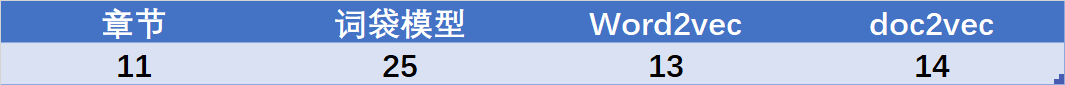
\includegraphics[width=0.8\linewidth]{figures/文档相似度.jpg}
    \caption{基于三种模型的文档相似度计算}
    \label{Doc}
\end{figure}

\subsubsection{文本聚类}
文本聚类指的是对文档进行聚类分析,被广泛用于文本挖掘和信息检索领域。

下面对整部《三体》利用k-means进行文本聚类,取其中最后五章的聚类结果进行展示,如图\ref{KMeans}:
\begin{figure}[!htbp]
    \centering
    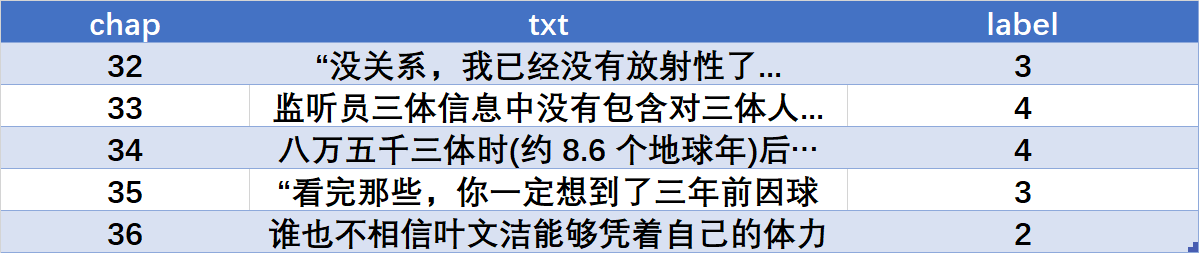
\includegraphics[width=0.8\linewidth]{figures/文本聚类.jpg}
    \caption{基于KMeans的文本聚类}
    \label{KMeans}
\end{figure}

\subsubsection{自动摘要}
自动摘要主要用于对文章提炼出主要内容,以摘要的形式供用户使用。

自动摘要的基本原理:文章的信息都包含在句子中,有些句子包含信息多,有些句子包含信息少。按照标点符号/分段符号,进行分句/分段。注意只使用“。!?”等确实代表整句结束的符号来分句。找出那些包含信息最多的句/段,将合并起来作为原文档的摘要。或者提取出其中所隐含的信息,用其生成文档的摘要。

下面对《三体》第一章进行自动摘要,结果如图\ref{abstract}。
\begin{figure}[!htbp]
    \centering
    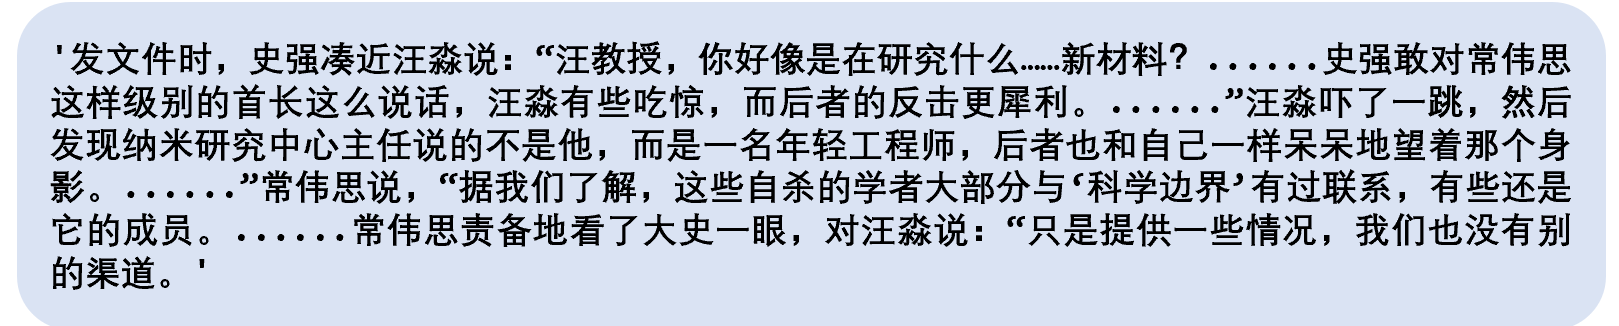
\includegraphics[width=\linewidth]{figures/自动摘要.png}
    \caption{对第一章进行自动摘要}
    \label{abstract}
\end{figure}

\subsection{情感分析}

情感分析(Sentiment Analysis)是对带有情感色彩的主观性文本进行分析、处理、归纳和推理的过程。

情感分析有三种常用的计算方法:

\begin{enumerate}
    \item 基于词典进行情感分析:
    
    根据情感词典对句子进行情感得分求和以得到情感倾向。

    \item 基于词袋模型进行情感分析:
    
    获取已准确分类的训练样本。以词袋模型为基础,将情感分析完全看作是文本分类的一个简单实例来进行处理。可按照分类进行预测,也可以按照情感值进行预测。效果优于词典模型,但仍然忽略了上下文的关联信息。

    \item 基于Word2Vec的情感分析:
    
    与词袋模型类似,只不过将此得表达方式改为Word2Vec。

\end{enumerate}

下面利用基于词典的方法,对《三体》中某些句子进行情感分析,我们用的情绪词典是清华大学李军中文褒贬义词典,结果如图\ref{score}。

\begin{figure}[b]
    \centering
    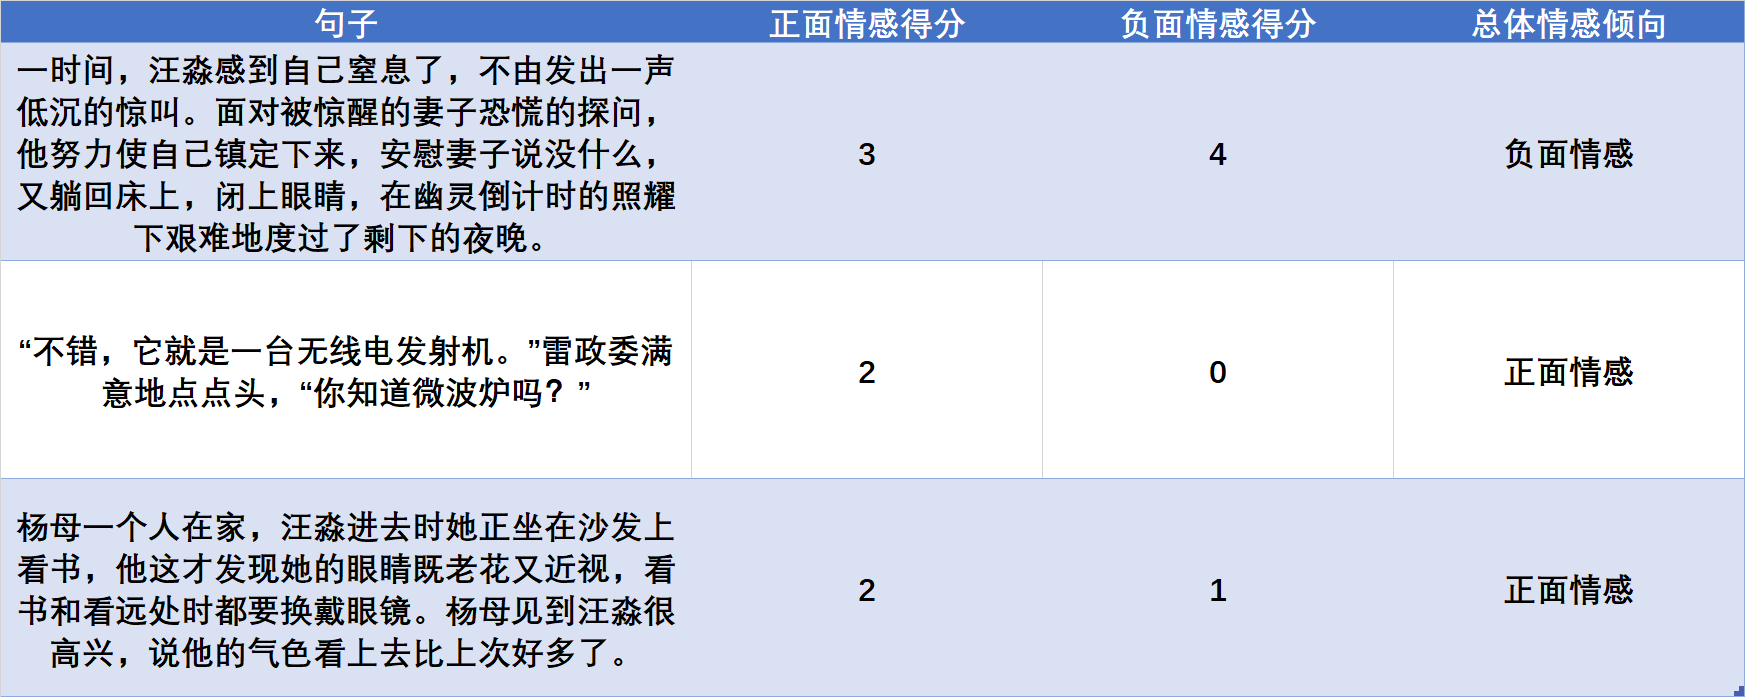
\includegraphics[width=0.9\linewidth]{figures/情感得分.jpg}
    \caption{例句情感得分}
    \label{score}
\end{figure}

可以发现基于词典的方法判断情感还是较为简单且可能存在较大误差的,因为词典仅仅能捕捉词本身,而无法考虑上下文的语境,因此效果可能不是很理想。

\subsection{自动写作}
自动写作是指人工智能算法自主完成写作任务,在写作过程中不需要人工干预。当前计算机已经能够自动撰写数据新闻、热点新闻、投研报告、联想式新闻等类型。

主要方法有利用逻辑回归(CNN)自动写作、利用 RNN 循环神经网络自动写作、利用 LSTM 自动写作,三种模型各有利弊;下面应用三种方法,利用了预训练的续写模型,对三体进行创意续写,我们的开头为:“三体来了!”如图\ref{autowriting}。

\begin{figure}[!htbp]
    \centering
    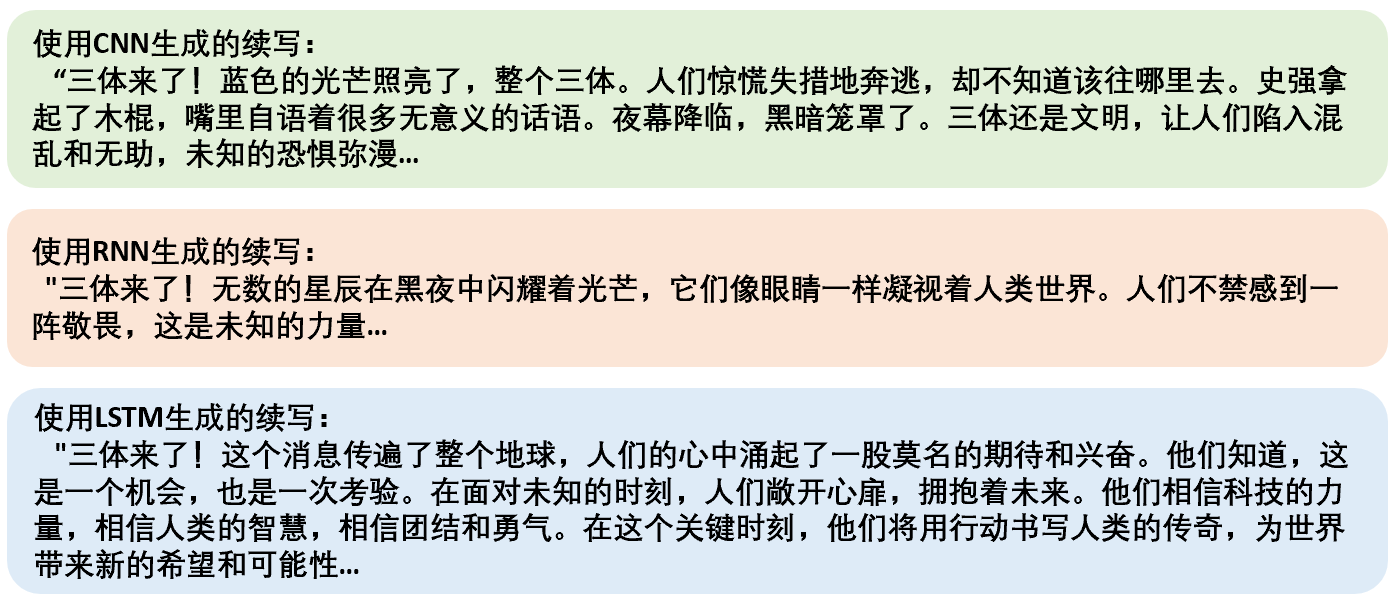
\includegraphics[width=0.9\linewidth]{figures/续写.png}
    \caption{利用三种模型续写结果展示}
    \label{autowriting}
\end{figure}

可以看出,CNN模型的训练效果不是很好,写出的内容比较混乱没有逻辑,而RNN和LSTM在经过大量文本训练后已能表现出相对高的写作水平,但是仍面对着字数过多后出现逻辑混乱、表达不清的现象。

\subsection{总结}
本研究项目旨在对《三体》文本进行细致的分析。首先,对三部曲进行了分词及词频统计,并通过词云可视化展示了词频分布情况。接着,基于不同的表示方法,探索了叶文洁、汪淼、丁仪以及三体等相关的词语,以更好地理解文章的关系,并对不同表示方法进行了比较。

在进一步分析中,本研究进行了文章的关键词提取与主题识别,提取出了每章的关键词,有助于理解每章的主要内容。随后,对文档相似性及其应用进行了研究,通过聚类和自动摘要的方法对文本进行了处理。

此外,本研究还利用情感词典的分析方法对《三体》文章中的句子进行了情感倾向判断,以揭示情感色彩在文本中的表达特征。最后,本研究还运用了CNN、RNN、LSTM等深度学习模型对《三体》进行了续写实验。通过这一步骤,进一步探索了文本生成和创作的可能性。

综上所述,本研究项目通过对《三体》文本的分词、词频统计、词云可视化、词语相似度、关键词提取、主题识别、文档相似性、情感分析以及文本生成等多个方面的研究,提供了对该文本的深入分析和理解。这些研究结果对于进一步挖掘《三体》以及其他文本作品的内涵和应用具有重要的参考价值。


% 在正文的最后添加 \newpage
\newpage
\thispagestyle{empty}

% 封底页内容

\begin{figure}[!htbp]
    \centering
    
\includegraphics[width=\linewidth]{figures/封底.png}
\end{figure}

\end{document}
